\documentclass[1p]{elsarticle_modified}
%\bibliographystyle{elsarticle-num}

%\usepackage[colorlinks]{hyperref}
%\usepackage{abbrmath_seonhwa} %\Abb, \Ascr, \Acal ,\Abf, \Afrak
\usepackage{amsfonts}
\usepackage{amssymb}
\usepackage{amsmath}
\usepackage{amsthm}
\usepackage{scalefnt}
\usepackage{amsbsy}
\usepackage{kotex}
\usepackage{caption}
\usepackage{subfig}
\usepackage{color}
\usepackage{graphicx}
\usepackage{xcolor} %% white, black, red, green, blue, cyan, magenta, yellow
\usepackage{float}
\usepackage{setspace}
\usepackage{hyperref}

\usepackage{tikz}
\usetikzlibrary{arrows}

\usepackage{multirow}
\usepackage{array} % fixed length table
\usepackage{hhline}

%%%%%%%%%%%%%%%%%%%%%
\makeatletter
\renewcommand*\env@matrix[1][\arraystretch]{%
	\edef\arraystretch{#1}%
	\hskip -\arraycolsep
	\let\@ifnextchar\new@ifnextchar
	\array{*\c@MaxMatrixCols c}}
\makeatother %https://tex.stackexchange.com/questions/14071/how-can-i-increase-the-line-spacing-in-a-matrix
%%%%%%%%%%%%%%%

\usepackage[normalem]{ulem}

\newcommand{\msout}[1]{\ifmmode\text{\sout{\ensuremath{#1}}}\else\sout{#1}\fi}
%SOURCE: \msout is \stkout macro in https://tex.stackexchange.com/questions/20609/strikeout-in-math-mode

\newcommand{\cancel}[1]{
	\ifmmode
	{\color{red}\msout{#1}}
	\else
	{\color{red}\sout{#1}}
	\fi
}

\newcommand{\add}[1]{
	{\color{blue}\uwave{#1}}
}

\newcommand{\replace}[2]{
	\ifmmode
	{\color{red}\msout{#1}}{\color{blue}\uwave{#2}}
	\else
	{\color{red}\sout{#1}}{\color{blue}\uwave{#2}}
	\fi
}

\newcommand{\Sol}{\mathcal{S}} %segment
\newcommand{\D}{D} %diagram
\newcommand{\A}{\mathcal{A}} %arc


%%%%%%%%%%%%%%%%%%%%%%%%%%%%%5 test

\def\sl{\operatorname{\textup{SL}}(2,\Cbb)}
\def\psl{\operatorname{\textup{PSL}}(2,\Cbb)}
\def\quan{\mkern 1mu \triangleright \mkern 1mu}

\theoremstyle{definition}
\newtheorem{thm}{Theorem}[section]
\newtheorem{prop}[thm]{Proposition}
\newtheorem{lem}[thm]{Lemma}
\newtheorem{ques}[thm]{Question}
\newtheorem{cor}[thm]{Corollary}
\newtheorem{defn}[thm]{Definition}
\newtheorem{exam}[thm]{Example}
\newtheorem{rmk}[thm]{Remark}
\newtheorem{alg}[thm]{Algorithm}

\newcommand{\I}{\sqrt{-1}}
\begin{document}

%\begin{frontmatter}
%
%\title{Boundary parabolic representations of knots up to 8 crossings}
%
%%% Group authors per affiliation:
%\author{Yunhi Cho} 
%\address{Department of Mathematics, University of Seoul, Seoul, Korea}
%\ead{yhcho@uos.ac.kr}
%
%
%\author{Seonhwa Kim} %\fnref{s_kim}}
%\address{Center for Geometry and Physics, Institute for Basic Science, Pohang, 37673, Korea}
%\ead{ryeona17@ibs.re.kr}
%
%\author{Hyuk Kim}
%\address{Department of Mathematical Sciences, Seoul National University, Seoul 08826, Korea}
%\ead{hyukkim@snu.ac.kr}
%
%\author{Seokbeom Yoon}
%\address{Department of Mathematical Sciences, Seoul National University, Seoul, 08826,  Korea}
%\ead{sbyoon15@snu.ac.kr}
%
%\begin{abstract}
%We find all boundary parabolic representation of knots up to 8 crossings.
%
%\end{abstract}
%\begin{keyword}
%    \MSC[2010] 57M25 
%\end{keyword}
%
%\end{frontmatter}

%\linenumbers
%\tableofcontents
%
\newcommand\colored[1]{\textcolor{white}{\rule[-0.35ex]{0.8em}{1.4ex}}\kern-0.8em\color{red} #1}%
%\newcommand\colored[1]{\textcolor{white}{ #1}\kern-2.17ex	\textcolor{white}{ #1}\kern-1.81ex	\textcolor{white}{ #1}\kern-2.15ex\color{red}#1	}

{\Large $\underline{12a_{0699}~(K12a_{0699})}$}

\setlength{\tabcolsep}{10pt}
\renewcommand{\arraystretch}{1.6}
\vspace{1cm}\begin{tabular}{m{100pt}>{\centering\arraybackslash}m{274pt}}
\multirow{5}{120pt}{
	\centering
	\includegraphics[width=112pt]{../../../GIT/diagram.site/Diagrams/png/1500_12a_0699.png}\\
\ \ \ A knot diagram\footnotemark}&
\allowdisplaybreaks
\textbf{Linearized knot diagam} \\
\cline{2-2}
 &
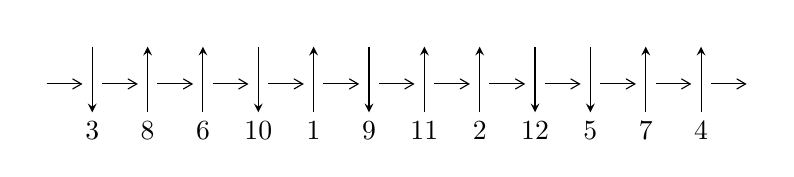
\begin{tikzpicture}[x=20pt, y=17pt]
	% nodes
	\node (C0) at (0, 0) {};
	\node (C1) at (1, 0) {};
	\node (C1U) at (1, +1) {};
	\node (C1D) at (1, -1) {3};

	\node (C2) at (2, 0) {};
	\node (C2U) at (2, +1) {};
	\node (C2D) at (2, -1) {8};

	\node (C3) at (3, 0) {};
	\node (C3U) at (3, +1) {};
	\node (C3D) at (3, -1) {6};

	\node (C4) at (4, 0) {};
	\node (C4U) at (4, +1) {};
	\node (C4D) at (4, -1) {10};

	\node (C5) at (5, 0) {};
	\node (C5U) at (5, +1) {};
	\node (C5D) at (5, -1) {1};

	\node (C6) at (6, 0) {};
	\node (C6U) at (6, +1) {};
	\node (C6D) at (6, -1) {9};

	\node (C7) at (7, 0) {};
	\node (C7U) at (7, +1) {};
	\node (C7D) at (7, -1) {11};

	\node (C8) at (8, 0) {};
	\node (C8U) at (8, +1) {};
	\node (C8D) at (8, -1) {2};

	\node (C9) at (9, 0) {};
	\node (C9U) at (9, +1) {};
	\node (C9D) at (9, -1) {12};

	\node (C10) at (10, 0) {};
	\node (C10U) at (10, +1) {};
	\node (C10D) at (10, -1) {5};

	\node (C11) at (11, 0) {};
	\node (C11U) at (11, +1) {};
	\node (C11D) at (11, -1) {7};

	\node (C12) at (12, 0) {};
	\node (C12U) at (12, +1) {};
	\node (C12D) at (12, -1) {4};
	\node (C13) at (13, 0) {};

	% arrows
	\draw[->,>={angle 60}]
	(C0) edge (C1) (C1) edge (C2) (C2) edge (C3) (C3) edge (C4) (C4) edge (C5) (C5) edge (C6) (C6) edge (C7) (C7) edge (C8) (C8) edge (C9) (C9) edge (C10) (C10) edge (C11) (C11) edge (C12) (C12) edge (C13) ;	\draw[->,>=stealth]
	(C1U) edge (C1D) (C2D) edge (C2U) (C3D) edge (C3U) (C4U) edge (C4D) (C5D) edge (C5U) (C6U) edge (C6D) (C7D) edge (C7U) (C8D) edge (C8U) (C9U) edge (C9D) (C10U) edge (C10D) (C11D) edge (C11U) (C12D) edge (C12U) ;
	\end{tikzpicture} \\
\hhline{~~} \\& 
\textbf{Solving Sequence} \\ \cline{2-2} 
 &
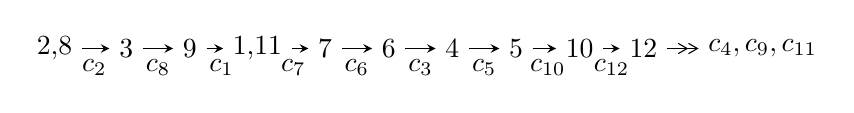
\begin{tikzpicture}[x=23pt, y=7pt]
	% node
	\node (A0) at (-1/8, 0) {2,8};
	\node (A1) at (1, 0) {3};
	\node (A2) at (2, 0) {9};
	\node (A3) at (49/16, 0) {1,11};
	\node (A4) at (33/8, 0) {7};
	\node (A5) at (41/8, 0) {6};
	\node (A6) at (49/8, 0) {4};
	\node (A7) at (57/8, 0) {5};
	\node (A8) at (65/8, 0) {10};
	\node (A9) at (73/8, 0) {12};
	\node (C1) at (1/2, -1) {$c_{2}$};
	\node (C2) at (3/2, -1) {$c_{8}$};
	\node (C3) at (5/2, -1) {$c_{1}$};
	\node (C4) at (29/8, -1) {$c_{7}$};
	\node (C5) at (37/8, -1) {$c_{6}$};
	\node (C6) at (45/8, -1) {$c_{3}$};
	\node (C7) at (53/8, -1) {$c_{5}$};
	\node (C8) at (61/8, -1) {$c_{10}$};
	\node (C9) at (69/8, -1) {$c_{12}$};
	\node (A10) at (11, 0) {$c_{4},c_{9},c_{11}$};

	% edge
	\draw[->,>=stealth]	
	(A0) edge (A1) (A1) edge (A2) (A2) edge (A3) (A3) edge (A4) (A4) edge (A5) (A5) edge (A6) (A6) edge (A7) (A7) edge (A8) (A8) edge (A9) ;
	\draw[->>,>={angle 60}]	
	(A9) edge (A10);
\end{tikzpicture} \\ 

\end{tabular} \\

\footnotetext{
The image of knot diagram is generated by the software ``\textbf{Draw programme}" developed by Andrew Bartholomew(\url{http://www.layer8.co.uk/maths/draw/index.htm\#Running-draw}), where we modified some parts for our purpose(\url{https://github.com/CATsTAILs/LinksPainter}).
}\phantom \\ \newline 
\centering \textbf{Ideals for irreducible components\footnotemark of $X_{\text{par}}$} 
 
\begin{align*}
I^u_{1}&=\langle 
-7.11942\times10^{639} u^{171}-2.78587\times10^{640} u^{170}+\cdots+7.11957\times10^{639} b-5.07255\times10^{642},\\
\phantom{I^u_{1}}&\phantom{= \langle  }-7.87299\times10^{640} u^{171}+1.65662\times10^{641} u^{170}+\cdots+1.58766\times10^{642} a+4.05831\times10^{644},\\
\phantom{I^u_{1}}&\phantom{= \langle  }u^{172}+4 u^{171}+\cdots+3076 u+892\rangle \\
I^u_{2}&=\langle 
-1.03311\times10^{27} u^{41}+2.27460\times10^{27} u^{40}+\cdots+6.16398\times10^{26} b-1.34436\times10^{27},\\
\phantom{I^u_{2}}&\phantom{= \langle  }-1.12761\times10^{27} u^{41}+5.58166\times10^{27} u^{40}+\cdots+1.23280\times10^{27} a+2.62673\times10^{28},\\
\phantom{I^u_{2}}&\phantom{= \langle  }u^{42}-3 u^{41}+\cdots-12 u+4\rangle \\
\\
\end{align*}
\raggedright * 2 irreducible components of $\dim_{\mathbb{C}}=0$, with total 214 representations.\\
\footnotetext{All coefficients of polynomials are rational numbers. But the coefficients are sometimes approximated in decimal forms when there is not enough margin.}
\newpage
\renewcommand{\arraystretch}{1}
\centering \section*{I. $I^u_{1}= \langle -7.12\times10^{639} u^{171}-2.79\times10^{640} u^{170}+\cdots+7.12\times10^{639} b-5.07\times10^{642},\;-7.87\times10^{640} u^{171}+1.66\times10^{641} u^{170}+\cdots+1.59\times10^{642} a+4.06\times10^{644},\;u^{172}+4 u^{171}+\cdots+3076 u+892 \rangle$}
\flushleft \textbf{(i) Arc colorings}\\
\begin{tabular}{m{7pt} m{180pt} m{7pt} m{180pt} }
\flushright $a_{2}=$&$\begin{pmatrix}1\\0\end{pmatrix}$ \\
\flushright $a_{8}=$&$\begin{pmatrix}0\\u\end{pmatrix}$ \\
\flushright $a_{3}=$&$\begin{pmatrix}1\\- u^2\end{pmatrix}$ \\
\flushright $a_{9}=$&$\begin{pmatrix}u\\u\end{pmatrix}$ \\
\flushright $a_{1}=$&$\begin{pmatrix}u^2+1\\- u^4\end{pmatrix}$ \\
\flushright $a_{11}=$&$\begin{pmatrix}0.0495885 u^{171}-0.104343 u^{170}+\cdots-649.335 u-255.615\\0.999979 u^{171}+3.91298 u^{170}+\cdots+2666.54 u+712.480\end{pmatrix}$ \\
\flushright $a_{7}=$&$\begin{pmatrix}0.665404 u^{171}+2.88035 u^{170}+\cdots+2516.78 u+747.159\\0.126747 u^{171}+1.77211 u^{170}+\cdots+3409.29 u+1301.02\end{pmatrix}$ \\
\flushright $a_{6}=$&$\begin{pmatrix}0.287095 u^{171}+0.685769 u^{170}+\cdots-221.459 u-186.229\\-0.251562 u^{171}-0.422463 u^{170}+\cdots+671.045 u+367.632\end{pmatrix}$ \\
\flushright $a_{4}=$&$\begin{pmatrix}0.342578 u^{171}+1.55098 u^{170}+\cdots+1632.44 u+505.425\\0.337631 u^{171}+1.40966 u^{170}+\cdots+1320.67 u+394.445\end{pmatrix}$ \\
\flushright $a_{5}=$&$\begin{pmatrix}0.544119 u^{171}+2.29704 u^{170}+\cdots+1923.71 u+555.144\\-0.235368 u^{171}+0.434597 u^{170}+\cdots+2601.45 u+1111.53\end{pmatrix}$ \\
\flushright $a_{10}=$&$\begin{pmatrix}-0.0899103 u^{171}-0.494492 u^{170}+\cdots-786.015 u-270.909\\0.825414 u^{171}+3.01234 u^{170}+\cdots+1579.13 u+313.228\end{pmatrix}$ \\
\flushright $a_{12}=$&$\begin{pmatrix}-0.406398 u^{171}-1.22172 u^{170}+\cdots-330.601 u+14.3430\\-0.116379 u^{171}-0.131742 u^{170}+\cdots+311.010 u+166.678\end{pmatrix}$\\&\end{tabular}
\flushleft \textbf{(ii) Obstruction class $= -1$}\\~\\
\flushleft \textbf{(iii) Cusp Shapes $= -0.257423 u^{171}-2.68415 u^{170}+\cdots-4456.58 u-1644.95$}\\~\\
\newpage\renewcommand{\arraystretch}{1}
\flushleft \textbf{(iv) u-Polynomials at the component}\newline \\
\begin{tabular}{m{50pt}|m{274pt}}
Crossings & \hspace{64pt}u-Polynomials at each crossing \\
\hline $$\begin{aligned}c_{1}\end{aligned}$$&$\begin{aligned}
&u^{172}+76 u^{171}+\cdots+25122848 u+795664
\end{aligned}$\\
\hline $$\begin{aligned}c_{2},c_{8}\end{aligned}$$&$\begin{aligned}
&u^{172}+4 u^{171}+\cdots+3076 u+892
\end{aligned}$\\
\hline $$\begin{aligned}c_{3}\end{aligned}$$&$\begin{aligned}
&81(81 u^{172}+2313 u^{171}+\cdots+27 u+1)
\end{aligned}$\\
\hline $$\begin{aligned}c_{4},c_{10}\end{aligned}$$&$\begin{aligned}
&9(9 u^{172}-21 u^{171}+\cdots+3804472 u+145372)
\end{aligned}$\\
\hline $$\begin{aligned}c_{5}\end{aligned}$$&$\begin{aligned}
&u^{172}-3 u^{171}+\cdots+1853937 u+164349
\end{aligned}$\\
\hline $$\begin{aligned}c_{6}\end{aligned}$$&$\begin{aligned}
&u^{172}-5 u^{171}+\cdots-7246383780 u+366700275
\end{aligned}$\\
\hline $$\begin{aligned}c_{7},c_{11}\end{aligned}$$&$\begin{aligned}
&9(9 u^{172}-30 u^{171}+\cdots+1621697 u+523514)
\end{aligned}$\\
\hline $$\begin{aligned}c_{9}\end{aligned}$$&$\begin{aligned}
&u^{172}-13 u^{171}+\cdots-15667632934 u+1387956497
\end{aligned}$\\
\hline $$\begin{aligned}c_{12}\end{aligned}$$&$\begin{aligned}
&u^{172}+17 u^{171}+\cdots+338848083 u+26871588
\end{aligned}$\\
\hline
\end{tabular}\\~\\
\newpage\renewcommand{\arraystretch}{1}
\flushleft \textbf{(v) Riley Polynomials at the component}\newline \\
\begin{tabular}{m{50pt}|m{274pt}}
Crossings & \hspace{64pt}Riley Polynomials at each crossing \\
\hline $$\begin{aligned}c_{1}\end{aligned}$$&$\begin{aligned}
&y^{172}+48 y^{171}+\cdots+43751823032704 y+633081200896
\end{aligned}$\\
\hline $$\begin{aligned}c_{2},c_{8}\end{aligned}$$&$\begin{aligned}
&y^{172}+76 y^{171}+\cdots+25122848 y+795664
\end{aligned}$\\
\hline $$\begin{aligned}c_{3}\end{aligned}$$&$\begin{aligned}
&6561(6561 y^{172}-327483 y^{171}+\cdots+571 y+1)
\end{aligned}$\\
\hline $$\begin{aligned}c_{4},c_{10}\end{aligned}$$&$\begin{aligned}
&81(81 y^{172}-9927 y^{171}+\cdots-4.86749\times10^{12} y+2.11330\times10^{10})
\end{aligned}$\\
\hline $$\begin{aligned}c_{5}\end{aligned}$$&$\begin{aligned}
&y^{172}-9 y^{171}+\cdots+646282891935 y+27010593801
\end{aligned}$\\
\hline $$\begin{aligned}c_{6}\end{aligned}$$&$\begin{aligned}
&y^{172}-23 y^{171}+\cdots-1.08\times10^{19} y+1.34\times10^{17}
\end{aligned}$\\
\hline $$\begin{aligned}c_{7},c_{11}\end{aligned}$$&$\begin{aligned}
&81(81 y^{172}+7650 y^{171}+\cdots+6.61151\times10^{12} y+2.74067\times10^{11})
\end{aligned}$\\
\hline $$\begin{aligned}c_{9}\end{aligned}$$&$\begin{aligned}
&y^{172}-63 y^{171}+\cdots-2.69\times10^{19} y+1.93\times10^{18}
\end{aligned}$\\
\hline $$\begin{aligned}c_{12}\end{aligned}$$&$\begin{aligned}
&y^{172}+31 y^{171}+\cdots+33369002886734055 y+722082241641744
\end{aligned}$\\
\hline
\end{tabular}\\~\\
\newpage\flushleft \textbf{(vi) Complex Volumes and Cusp Shapes}
$$\begin{array}{c|c|c}  
\text{Solutions to }I^u_{1}& \I (\text{vol} + \sqrt{-1}CS) & \text{Cusp shape}\\
 \hline 
\begin{aligned}
u &= -0.444314 + 0.896690 I \\
a &= \phantom{-}1.113900 + 0.174810 I \\
b &= \phantom{-}2.66959 - 1.09722 I\end{aligned}
 & -4.76658 - 4.24724 I & \phantom{-0.000000 } 0 \\ \hline\begin{aligned}
u &= -0.444314 - 0.896690 I \\
a &= \phantom{-}1.113900 - 0.174810 I \\
b &= \phantom{-}2.66959 + 1.09722 I\end{aligned}
 & -4.76658 + 4.24724 I & \phantom{-0.000000 } 0 \\ \hline\begin{aligned}
u &= -0.677854 + 0.721137 I \\
a &= \phantom{-}0.405323 + 0.565729 I \\
b &= \phantom{-}0.645666 + 0.622245 I\end{aligned}
 & \phantom{-}4.17273 - 0.06185 I & \phantom{-0.000000 } 0 \\ \hline\begin{aligned}
u &= -0.677854 - 0.721137 I \\
a &= \phantom{-}0.405323 - 0.565729 I \\
b &= \phantom{-}0.645666 - 0.622245 I\end{aligned}
 & \phantom{-}4.17273 + 0.06185 I & \phantom{-0.000000 } 0 \\ \hline\begin{aligned}
u &= -0.957946 + 0.326646 I \\
a &= -0.645620 + 0.881778 I \\
b &= -0.649863 - 0.453342 I\end{aligned}
 & -1.18665 - 3.57370 I & \phantom{-0.000000 } 0 \\ \hline\begin{aligned}
u &= -0.957946 - 0.326646 I \\
a &= -0.645620 - 0.881778 I \\
b &= -0.649863 + 0.453342 I\end{aligned}
 & -1.18665 + 3.57370 I & \phantom{-0.000000 } 0 \\ \hline\begin{aligned}
u &= \phantom{-}0.595294 + 0.786960 I \\
a &= \phantom{-}0.773630 - 0.035104 I \\
b &= \phantom{-}0.627151 + 0.821745 I\end{aligned}
 & \phantom{-}0.88993 + 1.85918 I & \phantom{-0.000000 } 0 \\ \hline\begin{aligned}
u &= \phantom{-}0.595294 - 0.786960 I \\
a &= \phantom{-}0.773630 + 0.035104 I \\
b &= \phantom{-}0.627151 - 0.821745 I\end{aligned}
 & \phantom{-}0.88993 - 1.85918 I & \phantom{-0.000000 } 0 \\ \hline\begin{aligned}
u &= \phantom{-}0.922311 + 0.350507 I \\
a &= \phantom{-}0.138078 + 0.904791 I \\
b &= \phantom{-}0.436870 - 0.791878 I\end{aligned}
 & \phantom{-}1.64081 - 1.77100 I & \phantom{-0.000000 } 0 \\ \hline\begin{aligned}
u &= \phantom{-}0.922311 - 0.350507 I \\
a &= \phantom{-}0.138078 - 0.904791 I \\
b &= \phantom{-}0.436870 + 0.791878 I\end{aligned}
 & \phantom{-}1.64081 + 1.77100 I & \phantom{-0.000000 } 0\\
 \hline 
 \end{array}$$\newpage$$\begin{array}{c|c|c}  
\text{Solutions to }I^u_{1}& \I (\text{vol} + \sqrt{-1}CS) & \text{Cusp shape}\\
 \hline 
\begin{aligned}
u &= \phantom{-}0.504799 + 0.880123 I \\
a &= \phantom{-}1.57977 - 1.78074 I \\
b &= \phantom{-}1.82823 - 1.63741 I\end{aligned}
 & -1.62431 + 2.07905 I & \phantom{-0.000000 } 0 \\ \hline\begin{aligned}
u &= \phantom{-}0.504799 - 0.880123 I \\
a &= \phantom{-}1.57977 + 1.78074 I \\
b &= \phantom{-}1.82823 + 1.63741 I\end{aligned}
 & -1.62431 - 2.07905 I & \phantom{-0.000000 } 0 \\ \hline\begin{aligned}
u &= -0.775463 + 0.607818 I \\
a &= -0.785572 - 0.443717 I \\
b &= -0.666606 + 0.025546 I\end{aligned}
 & \phantom{-}3.02226 + 3.08004 I & \phantom{-0.000000 } 0 \\ \hline\begin{aligned}
u &= -0.775463 - 0.607818 I \\
a &= -0.785572 + 0.443717 I \\
b &= -0.666606 - 0.025546 I\end{aligned}
 & \phantom{-}3.02226 - 3.08004 I & \phantom{-0.000000 } 0 \\ \hline\begin{aligned}
u &= -0.918010 + 0.344848 I \\
a &= -0.168441 - 0.974586 I \\
b &= -0.088221 + 0.940929 I\end{aligned}
 & \phantom{-}0.83568 + 5.69605 I & \phantom{-0.000000 } 0 \\ \hline\begin{aligned}
u &= -0.918010 - 0.344848 I \\
a &= -0.168441 + 0.974586 I \\
b &= -0.088221 - 0.940929 I\end{aligned}
 & \phantom{-}0.83568 - 5.69605 I & \phantom{-0.000000 } 0 \\ \hline\begin{aligned}
u &= \phantom{-}0.863576 + 0.542838 I \\
a &= \phantom{-}0.870045 + 0.274052 I \\
b &= \phantom{-}0.565989 - 0.009645 I\end{aligned}
 & \phantom{-}1.22443 - 1.30449 I & \phantom{-0.000000 } 0 \\ \hline\begin{aligned}
u &= \phantom{-}0.863576 - 0.542838 I \\
a &= \phantom{-}0.870045 - 0.274052 I \\
b &= \phantom{-}0.565989 + 0.009645 I\end{aligned}
 & \phantom{-}1.22443 + 1.30449 I & \phantom{-0.000000 } 0 \\ \hline\begin{aligned}
u &= -0.438231 + 0.875440 I \\
a &= \phantom{-}0.283520 - 1.028340 I \\
b &= -1.046310 - 0.298808 I\end{aligned}
 & -4.68377 + 0.63646 I & \phantom{-0.000000 } 0 \\ \hline\begin{aligned}
u &= -0.438231 - 0.875440 I \\
a &= \phantom{-}0.283520 + 1.028340 I \\
b &= -1.046310 + 0.298808 I\end{aligned}
 & -4.68377 - 0.63646 I & \phantom{-0.000000 } 0\\
 \hline 
 \end{array}$$\newpage$$\begin{array}{c|c|c}  
\text{Solutions to }I^u_{1}& \I (\text{vol} + \sqrt{-1}CS) & \text{Cusp shape}\\
 \hline 
\begin{aligned}
u &= -0.335203 + 0.918267 I \\
a &= \phantom{-}0.352550 + 0.576852 I \\
b &= -0.380013 - 0.337924 I\end{aligned}
 & -2.95880 + 2.07571 I & \phantom{-0.000000 } 0 \\ \hline\begin{aligned}
u &= -0.335203 - 0.918267 I \\
a &= \phantom{-}0.352550 - 0.576852 I \\
b &= -0.380013 + 0.337924 I\end{aligned}
 & -2.95880 - 2.07571 I & \phantom{-0.000000 } 0 \\ \hline\begin{aligned}
u &= \phantom{-}0.345935 + 0.964013 I \\
a &= -1.032810 - 0.922639 I \\
b &= -2.23306 - 0.29354 I\end{aligned}
 & -7.39431 + 0.13825 I & \phantom{-0.000000 } 0 \\ \hline\begin{aligned}
u &= \phantom{-}0.345935 - 0.964013 I \\
a &= -1.032810 + 0.922639 I \\
b &= -2.23306 + 0.29354 I\end{aligned}
 & -7.39431 - 0.13825 I & \phantom{-0.000000 } 0 \\ \hline\begin{aligned}
u &= \phantom{-}0.517845 + 0.820411 I \\
a &= -0.687604 - 0.880904 I \\
b &= -0.611455 + 1.264570 I\end{aligned}
 & \phantom{-}0.817136 + 1.106290 I & \phantom{-0.000000 } 0 \\ \hline\begin{aligned}
u &= \phantom{-}0.517845 - 0.820411 I \\
a &= -0.687604 + 0.880904 I \\
b &= -0.611455 - 1.264570 I\end{aligned}
 & \phantom{-}0.817136 - 1.106290 I & \phantom{-0.000000 } 0 \\ \hline\begin{aligned}
u &= -0.680910 + 0.690973 I \\
a &= \phantom{-}0.327286 - 1.001280 I \\
b &= -0.674580 + 0.669526 I\end{aligned}
 & \phantom{-}0.01320 + 2.08002 I & \phantom{-0.000000 } 0 \\ \hline\begin{aligned}
u &= -0.680910 - 0.690973 I \\
a &= \phantom{-}0.327286 + 1.001280 I \\
b &= -0.674580 - 0.669526 I\end{aligned}
 & \phantom{-}0.01320 - 2.08002 I & \phantom{-0.000000 } 0 \\ \hline\begin{aligned}
u &= \phantom{-}0.448811 + 0.853822 I \\
a &= \phantom{-}0.985866 + 0.278785 I \\
b &= \phantom{-}2.51959 + 1.06869 I\end{aligned}
 & \phantom{-}0.017064 + 1.122660 I & \phantom{-0.000000 } 0 \\ \hline\begin{aligned}
u &= \phantom{-}0.448811 - 0.853822 I \\
a &= \phantom{-}0.985866 - 0.278785 I \\
b &= \phantom{-}2.51959 - 1.06869 I\end{aligned}
 & \phantom{-}0.017064 - 1.122660 I & \phantom{-0.000000 } 0\\
 \hline 
 \end{array}$$\newpage$$\begin{array}{c|c|c}  
\text{Solutions to }I^u_{1}& \I (\text{vol} + \sqrt{-1}CS) & \text{Cusp shape}\\
 \hline 
\begin{aligned}
u &= \phantom{-}0.713920 + 0.751808 I \\
a &= -0.600950 - 0.769742 I \\
b &= \phantom{-}0.826454 - 0.958050 I\end{aligned}
 & -2.49145 - 4.60127 I & \phantom{-0.000000 } 0 \\ \hline\begin{aligned}
u &= \phantom{-}0.713920 - 0.751808 I \\
a &= -0.600950 + 0.769742 I \\
b &= \phantom{-}0.826454 + 0.958050 I\end{aligned}
 & -2.49145 + 4.60127 I & \phantom{-0.000000 } 0 \\ \hline\begin{aligned}
u &= \phantom{-}0.526737 + 0.893857 I \\
a &= -1.048730 - 0.367243 I \\
b &= -3.28141 - 0.07709 I\end{aligned}
 & \phantom{-}0.56641 + 3.12116 I & \phantom{-0.000000 } 0 \\ \hline\begin{aligned}
u &= \phantom{-}0.526737 - 0.893857 I \\
a &= -1.048730 + 0.367243 I \\
b &= -3.28141 + 0.07709 I\end{aligned}
 & \phantom{-}0.56641 - 3.12116 I & \phantom{-0.000000 } 0 \\ \hline\begin{aligned}
u &= -0.141666 + 1.028690 I \\
a &= -0.250314 - 0.119199 I \\
b &= -0.87760 - 1.18524 I\end{aligned}
 & -5.97488 + 0.13240 I & \phantom{-0.000000 } 0 \\ \hline\begin{aligned}
u &= -0.141666 - 1.028690 I \\
a &= -0.250314 + 0.119199 I \\
b &= -0.87760 + 1.18524 I\end{aligned}
 & -5.97488 - 0.13240 I & \phantom{-0.000000 } 0 \\ \hline\begin{aligned}
u &= \phantom{-}0.895020 + 0.528313 I \\
a &= -0.182144 - 1.282520 I \\
b &= \phantom{-}0.034532 + 0.643268 I\end{aligned}
 & -0.37073 - 8.17547 I & \phantom{-0.000000 } 0 \\ \hline\begin{aligned}
u &= \phantom{-}0.895020 - 0.528313 I \\
a &= -0.182144 + 1.282520 I \\
b &= \phantom{-}0.034532 - 0.643268 I\end{aligned}
 & -0.37073 + 8.17547 I & \phantom{-0.000000 } 0 \\ \hline\begin{aligned}
u &= \phantom{-}0.770491 + 0.573420 I \\
a &= \phantom{-}1.091530 - 0.128106 I \\
b &= \phantom{-}1.059010 + 0.053499 I\end{aligned}
 & \phantom{-}2.47051 + 2.46378 I & \phantom{-0.000000 } 0 \\ \hline\begin{aligned}
u &= \phantom{-}0.770491 - 0.573420 I \\
a &= \phantom{-}1.091530 + 0.128106 I \\
b &= \phantom{-}1.059010 - 0.053499 I\end{aligned}
 & \phantom{-}2.47051 - 2.46378 I & \phantom{-0.000000 } 0\\
 \hline 
 \end{array}$$\newpage$$\begin{array}{c|c|c}  
\text{Solutions to }I^u_{1}& \I (\text{vol} + \sqrt{-1}CS) & \text{Cusp shape}\\
 \hline 
\begin{aligned}
u &= -0.916707 + 0.490817 I \\
a &= -0.005551 - 1.190440 I \\
b &= -0.252125 + 0.527816 I\end{aligned}
 & \phantom{-}0.63068 + 3.00510 I & \phantom{-0.000000 } 0 \\ \hline\begin{aligned}
u &= -0.916707 - 0.490817 I \\
a &= -0.005551 + 1.190440 I \\
b &= -0.252125 - 0.527816 I\end{aligned}
 & \phantom{-}0.63068 - 3.00510 I & \phantom{-0.000000 } 0 \\ \hline\begin{aligned}
u &= \phantom{-}0.825637 + 0.472579 I \\
a &= -1.142920 + 0.377601 I \\
b &= -0.928136 + 0.049806 I\end{aligned}
 & -0.52169 - 8.45025 I & \phantom{-0.000000 } 0 \\ \hline\begin{aligned}
u &= \phantom{-}0.825637 - 0.472579 I \\
a &= -1.142920 - 0.377601 I \\
b &= -0.928136 - 0.049806 I\end{aligned}
 & -0.52169 + 8.45025 I & \phantom{-0.000000 } 0 \\ \hline\begin{aligned}
u &= \phantom{-}0.066014 + 1.047780 I \\
a &= -0.146720 + 0.681990 I \\
b &= -0.033766 + 0.628880 I\end{aligned}
 & -2.79005 + 2.53157 I & \phantom{-0.000000 } 0 \\ \hline\begin{aligned}
u &= \phantom{-}0.066014 - 1.047780 I \\
a &= -0.146720 - 0.681990 I \\
b &= -0.033766 - 0.628880 I\end{aligned}
 & -2.79005 - 2.53157 I & \phantom{-0.000000 } 0 \\ \hline\begin{aligned}
u &= \phantom{-}0.483322 + 0.932023 I \\
a &= \phantom{-}0.258193 + 0.772674 I \\
b &= -0.108470 - 0.108813 I\end{aligned}
 & -0.31059 + 2.59895 I & \phantom{-0.000000 } 0 \\ \hline\begin{aligned}
u &= \phantom{-}0.483322 - 0.932023 I \\
a &= \phantom{-}0.258193 - 0.772674 I \\
b &= -0.108470 + 0.108813 I\end{aligned}
 & -0.31059 - 2.59895 I & \phantom{-0.000000 } 0 \\ \hline\begin{aligned}
u &= \phantom{-}0.492063 + 0.809699 I \\
a &= -0.59461 + 1.53435 I \\
b &= -0.606376 + 0.926960 I\end{aligned}
 & -1.41878 + 2.03132 I & \phantom{-0.000000 } 0 \\ \hline\begin{aligned}
u &= \phantom{-}0.492063 - 0.809699 I \\
a &= -0.59461 - 1.53435 I \\
b &= -0.606376 - 0.926960 I\end{aligned}
 & -1.41878 - 2.03132 I & \phantom{-0.000000 } 0\\
 \hline 
 \end{array}$$\newpage$$\begin{array}{c|c|c}  
\text{Solutions to }I^u_{1}& \I (\text{vol} + \sqrt{-1}CS) & \text{Cusp shape}\\
 \hline 
\begin{aligned}
u &= -0.494341 + 0.931042 I \\
a &= -0.471579 + 0.598238 I \\
b &= \phantom{-}0.06205 - 1.89940 I\end{aligned}
 & -2.32153 - 7.32120 I & \phantom{-0.000000 } 0 \\ \hline\begin{aligned}
u &= -0.494341 - 0.931042 I \\
a &= -0.471579 - 0.598238 I \\
b &= \phantom{-}0.06205 + 1.89940 I\end{aligned}
 & -2.32153 + 7.32120 I & \phantom{-0.000000 } 0 \\ \hline\begin{aligned}
u &= -0.250076 + 0.907912 I \\
a &= \phantom{-}1.45144 - 0.85887 I \\
b &= \phantom{-}2.20724 - 0.96331 I\end{aligned}
 & -7.40070 + 5.79515 I & \phantom{-0.000000 } 0 \\ \hline\begin{aligned}
u &= -0.250076 - 0.907912 I \\
a &= \phantom{-}1.45144 + 0.85887 I \\
b &= \phantom{-}2.20724 + 0.96331 I\end{aligned}
 & -7.40070 - 5.79515 I & \phantom{-0.000000 } 0 \\ \hline\begin{aligned}
u &= -0.453438 + 0.810747 I \\
a &= -0.855395 + 0.376915 I \\
b &= -3.97782 + 0.23710 I\end{aligned}
 & -1.86220 + 3.43609 I & \phantom{-0.000000 } 0 \\ \hline\begin{aligned}
u &= -0.453438 - 0.810747 I \\
a &= -0.855395 - 0.376915 I \\
b &= -3.97782 - 0.23710 I\end{aligned}
 & -1.86220 - 3.43609 I & \phantom{-0.000000 } 0 \\ \hline\begin{aligned}
u &= -0.500829 + 0.961519 I \\
a &= -0.456635 - 0.650896 I \\
b &= -0.513687 - 0.947118 I\end{aligned}
 & -3.89524 - 5.47159 I & \phantom{-0.000000 } 0 \\ \hline\begin{aligned}
u &= -0.500829 - 0.961519 I \\
a &= -0.456635 + 0.650896 I \\
b &= -0.513687 + 0.947118 I\end{aligned}
 & -3.89524 + 5.47159 I & \phantom{-0.000000 } 0 \\ \hline\begin{aligned}
u &= -0.687457 + 0.852804 I \\
a &= -0.640423 + 0.466864 I \\
b &= \phantom{-}0.65771 + 1.71387 I\end{aligned}
 & \phantom{-}2.36278 - 2.64451 I & \phantom{-0.000000 } 0 \\ \hline\begin{aligned}
u &= -0.687457 - 0.852804 I \\
a &= -0.640423 - 0.466864 I \\
b &= \phantom{-}0.65771 - 1.71387 I\end{aligned}
 & \phantom{-}2.36278 + 2.64451 I & \phantom{-0.000000 } 0\\
 \hline 
 \end{array}$$\newpage$$\begin{array}{c|c|c}  
\text{Solutions to }I^u_{1}& \I (\text{vol} + \sqrt{-1}CS) & \text{Cusp shape}\\
 \hline 
\begin{aligned}
u &= -0.983258 + 0.491988 I \\
a &= -0.030148 + 1.309630 I \\
b &= \phantom{-}0.184575 - 0.506908 I\end{aligned}
 & -3.9406 + 14.6159 I & \phantom{-0.000000 } 0 \\ \hline\begin{aligned}
u &= -0.983258 - 0.491988 I \\
a &= -0.030148 - 1.309630 I \\
b &= \phantom{-}0.184575 + 0.506908 I\end{aligned}
 & -3.9406 - 14.6159 I & \phantom{-0.000000 } 0 \\ \hline\begin{aligned}
u &= -0.608206 + 0.920459 I \\
a &= \phantom{-}0.909484 - 0.146029 I \\
b &= \phantom{-}2.83949 - 1.09248 I\end{aligned}
 & -0.65442 - 7.07658 I & \phantom{-0.000000 } 0 \\ \hline\begin{aligned}
u &= -0.608206 - 0.920459 I \\
a &= \phantom{-}0.909484 + 0.146029 I \\
b &= \phantom{-}2.83949 + 1.09248 I\end{aligned}
 & -0.65442 + 7.07658 I & \phantom{-0.000000 } 0 \\ \hline\begin{aligned}
u &= \phantom{-}1.043730 + 0.400521 I \\
a &= -0.002038 + 1.272240 I \\
b &= -0.130457 - 0.265102 I\end{aligned}
 & -0.75717 - 5.35150 I & \phantom{-0.000000 } 0 \\ \hline\begin{aligned}
u &= \phantom{-}1.043730 - 0.400521 I \\
a &= -0.002038 - 1.272240 I \\
b &= -0.130457 + 0.265102 I\end{aligned}
 & -0.75717 + 5.35150 I & \phantom{-0.000000 } 0 \\ \hline\begin{aligned}
u &= -0.443758 + 1.029070 I \\
a &= -0.812766 + 0.575345 I \\
b &= -2.10372 + 0.01711 I\end{aligned}
 & -4.04121 - 1.06499 I & \phantom{-0.000000 } 0 \\ \hline\begin{aligned}
u &= -0.443758 - 1.029070 I \\
a &= -0.812766 - 0.575345 I \\
b &= -2.10372 - 0.01711 I\end{aligned}
 & -4.04121 + 1.06499 I & \phantom{-0.000000 } 0 \\ \hline\begin{aligned}
u &= \phantom{-}0.550328 + 0.976342 I \\
a &= \phantom{-}1.220270 - 0.061283 I \\
b &= \phantom{-}2.46456 + 0.96409 I\end{aligned}
 & -6.08593 + 5.33871 I & \phantom{-0.000000 } 0 \\ \hline\begin{aligned}
u &= \phantom{-}0.550328 - 0.976342 I \\
a &= \phantom{-}1.220270 + 0.061283 I \\
b &= \phantom{-}2.46456 - 0.96409 I\end{aligned}
 & -6.08593 - 5.33871 I & \phantom{-0.000000 } 0\\
 \hline 
 \end{array}$$\newpage$$\begin{array}{c|c|c}  
\text{Solutions to }I^u_{1}& \I (\text{vol} + \sqrt{-1}CS) & \text{Cusp shape}\\
 \hline 
\begin{aligned}
u &= \phantom{-}0.534046 + 0.687237 I \\
a &= \phantom{-}0.488493 + 1.308980 I \\
b &= -0.825614 + 0.285354 I\end{aligned}
 & -5.15017 - 0.92884 I & \phantom{-0.000000 } 0 \\ \hline\begin{aligned}
u &= \phantom{-}0.534046 - 0.687237 I \\
a &= \phantom{-}0.488493 - 1.308980 I \\
b &= -0.825614 - 0.285354 I\end{aligned}
 & -5.15017 + 0.92884 I & \phantom{-0.000000 } 0 \\ \hline\begin{aligned}
u &= \phantom{-}0.639818 + 0.932642 I \\
a &= \phantom{-}0.065731 + 0.670333 I \\
b &= -0.611179 + 0.503384 I\end{aligned}
 & \phantom{-}0.42180 + 3.01163 I & \phantom{-0.000000 } 0 \\ \hline\begin{aligned}
u &= \phantom{-}0.639818 - 0.932642 I \\
a &= \phantom{-}0.065731 - 0.670333 I \\
b &= -0.611179 - 0.503384 I\end{aligned}
 & \phantom{-}0.42180 - 3.01163 I & \phantom{-0.000000 } 0 \\ \hline\begin{aligned}
u &= -0.593721 + 0.621763 I \\
a &= -0.49669 + 1.63921 I \\
b &= -0.021292 + 0.181530 I\end{aligned}
 & -4.13144 + 6.46662 I & \phantom{-0.000000 } 0 \\ \hline\begin{aligned}
u &= -0.593721 - 0.621763 I \\
a &= -0.49669 - 1.63921 I \\
b &= -0.021292 - 0.181530 I\end{aligned}
 & -4.13144 - 6.46662 I & \phantom{-0.000000 } 0 \\ \hline\begin{aligned}
u &= -0.640769 + 0.946193 I \\
a &= -0.542601 - 0.438875 I \\
b &= -0.452294 + 0.070085 I\end{aligned}
 & \phantom{-}3.48415 - 5.05283 I & \phantom{-0.000000 } 0 \\ \hline\begin{aligned}
u &= -0.640769 - 0.946193 I \\
a &= -0.542601 + 0.438875 I \\
b &= -0.452294 - 0.070085 I\end{aligned}
 & \phantom{-}3.48415 + 5.05283 I & \phantom{-0.000000 } 0 \\ \hline\begin{aligned}
u &= -0.636379 + 0.567392 I \\
a &= \phantom{-}0.236798 - 1.099070 I \\
b &= -0.382560 + 0.366833 I\end{aligned}
 & \phantom{-}0.17613 + 1.99144 I & \phantom{-0.000000 } 0 \\ \hline\begin{aligned}
u &= -0.636379 - 0.567392 I \\
a &= \phantom{-}0.236798 + 1.099070 I \\
b &= -0.382560 - 0.366833 I\end{aligned}
 & \phantom{-}0.17613 - 1.99144 I & \phantom{-0.000000 } 0\\
 \hline 
 \end{array}$$\newpage$$\begin{array}{c|c|c}  
\text{Solutions to }I^u_{1}& \I (\text{vol} + \sqrt{-1}CS) & \text{Cusp shape}\\
 \hline 
\begin{aligned}
u &= -0.581960 + 0.991557 I \\
a &= -1.42283 + 0.05743 I \\
b &= -2.72033 + 0.32539 I\end{aligned}
 & -5.24765 - 11.16740 I & \phantom{-0.000000 } 0 \\ \hline\begin{aligned}
u &= -0.581960 - 0.991557 I \\
a &= -1.42283 - 0.05743 I \\
b &= -2.72033 - 0.32539 I\end{aligned}
 & -5.24765 + 11.16740 I & \phantom{-0.000000 } 0 \\ \hline\begin{aligned}
u &= \phantom{-}0.666047 + 0.938720 I \\
a &= -0.826880 - 0.303795 I \\
b &= -0.56790 - 1.81639 I\end{aligned}
 & -3.06633 + 9.89751 I & \phantom{-0.000000 } 0 \\ \hline\begin{aligned}
u &= \phantom{-}0.666047 - 0.938720 I \\
a &= -0.826880 + 0.303795 I \\
b &= -0.56790 + 1.81639 I\end{aligned}
 & -3.06633 - 9.89751 I & \phantom{-0.000000 } 0 \\ \hline\begin{aligned}
u &= -0.063640 + 1.150590 I \\
a &= -0.917822 + 0.379717 I \\
b &= -2.67930 - 0.03013 I\end{aligned}
 & -5.70391 + 1.36026 I & \phantom{-0.000000 } 0 \\ \hline\begin{aligned}
u &= -0.063640 - 1.150590 I \\
a &= -0.917822 - 0.379717 I \\
b &= -2.67930 + 0.03013 I\end{aligned}
 & -5.70391 - 1.36026 I & \phantom{-0.000000 } 0 \\ \hline\begin{aligned}
u &= -0.149823 + 1.151860 I \\
a &= \phantom{-}1.137490 - 0.237386 I \\
b &= \phantom{-}2.86725 - 0.57716 I\end{aligned}
 & -11.44810 + 0.42410 I & \phantom{-0.000000 } 0 \\ \hline\begin{aligned}
u &= -0.149823 - 1.151860 I \\
a &= \phantom{-}1.137490 + 0.237386 I \\
b &= \phantom{-}2.86725 + 0.57716 I\end{aligned}
 & -11.44810 - 0.42410 I & \phantom{-0.000000 } 0 \\ \hline\begin{aligned}
u &= -0.912722 + 0.726373 I \\
a &= \phantom{-}0.526428 - 0.541434 I \\
b &= \phantom{-}0.338926 - 0.134167 I\end{aligned}
 & \phantom{-}2.03330 + 0.16994 I & \phantom{-0.000000 } 0 \\ \hline\begin{aligned}
u &= -0.912722 - 0.726373 I \\
a &= \phantom{-}0.526428 + 0.541434 I \\
b &= \phantom{-}0.338926 + 0.134167 I\end{aligned}
 & \phantom{-}2.03330 - 0.16994 I & \phantom{-0.000000 } 0\\
 \hline 
 \end{array}$$\newpage$$\begin{array}{c|c|c}  
\text{Solutions to }I^u_{1}& \I (\text{vol} + \sqrt{-1}CS) & \text{Cusp shape}\\
 \hline 
\begin{aligned}
u &= \phantom{-}0.510475 + 1.062640 I \\
a &= \phantom{-}1.124650 + 0.115723 I \\
b &= \phantom{-}3.43709 + 0.05722 I\end{aligned}
 & -7.89103 + 10.03170 I & \phantom{-0.000000 } 0 \\ \hline\begin{aligned}
u &= \phantom{-}0.510475 - 1.062640 I \\
a &= \phantom{-}1.124650 - 0.115723 I \\
b &= \phantom{-}3.43709 - 0.05722 I\end{aligned}
 & -7.89103 - 10.03170 I & \phantom{-0.000000 } 0 \\ \hline\begin{aligned}
u &= \phantom{-}0.086602 + 1.178420 I \\
a &= -0.075206 - 0.992788 I \\
b &= \phantom{-}0.281628 - 0.697506 I\end{aligned}
 & -6.14702 - 6.30554 I & \phantom{-0.000000 } 0 \\ \hline\begin{aligned}
u &= \phantom{-}0.086602 - 1.178420 I \\
a &= -0.075206 + 0.992788 I \\
b &= \phantom{-}0.281628 + 0.697506 I\end{aligned}
 & -6.14702 + 6.30554 I & \phantom{-0.000000 } 0 \\ \hline\begin{aligned}
u &= -0.765738 + 0.904306 I \\
a &= -0.376451 + 0.390915 I \\
b &= -0.330694 - 0.884347 I\end{aligned}
 & -2.78263 - 4.87703 I & \phantom{-0.000000 } 0 \\ \hline\begin{aligned}
u &= -0.765738 - 0.904306 I \\
a &= -0.376451 - 0.390915 I \\
b &= -0.330694 + 0.884347 I\end{aligned}
 & -2.78263 + 4.87703 I & \phantom{-0.000000 } 0 \\ \hline\begin{aligned}
u &= -0.642305 + 1.004790 I \\
a &= \phantom{-}0.860395 - 0.045405 I \\
b &= \phantom{-}2.00356 - 0.77879 I\end{aligned}
 & -1.02976 - 7.05861 I & \phantom{-0.000000 } 0 \\ \hline\begin{aligned}
u &= -0.642305 - 1.004790 I \\
a &= \phantom{-}0.860395 + 0.045405 I \\
b &= \phantom{-}2.00356 + 0.77879 I\end{aligned}
 & -1.02976 + 7.05861 I & \phantom{-0.000000 } 0 \\ \hline\begin{aligned}
u &= \phantom{-}0.347976 + 1.152370 I \\
a &= -0.848161 - 0.539875 I \\
b &= -2.61179 - 0.70726 I\end{aligned}
 & -8.96205 - 2.66335 I & \phantom{-0.000000 } 0 \\ \hline\begin{aligned}
u &= \phantom{-}0.347976 - 1.152370 I \\
a &= -0.848161 + 0.539875 I \\
b &= -2.61179 + 0.70726 I\end{aligned}
 & -8.96205 + 2.66335 I & \phantom{-0.000000 } 0\\
 \hline 
 \end{array}$$\newpage$$\begin{array}{c|c|c}  
\text{Solutions to }I^u_{1}& \I (\text{vol} + \sqrt{-1}CS) & \text{Cusp shape}\\
 \hline 
\begin{aligned}
u &= -0.045994 + 1.208720 I \\
a &= \phantom{-}1.050720 + 0.240655 I \\
b &= \phantom{-}2.84566 + 0.14258 I\end{aligned}
 & -6.97404 - 6.28993 I & \phantom{-0.000000 } 0 \\ \hline\begin{aligned}
u &= -0.045994 - 1.208720 I \\
a &= \phantom{-}1.050720 - 0.240655 I \\
b &= \phantom{-}2.84566 - 0.14258 I\end{aligned}
 & -6.97404 + 6.28993 I & \phantom{-0.000000 } 0 \\ \hline\begin{aligned}
u &= -0.782595 + 0.049312 I \\
a &= \phantom{-}0.46790 - 1.74852 I \\
b &= \phantom{-}0.432361 - 0.211392 I\end{aligned}
 & -6.35993 + 3.64195 I & \phantom{-0.000000 } 0 \\ \hline\begin{aligned}
u &= -0.782595 - 0.049312 I \\
a &= \phantom{-}0.46790 + 1.74852 I \\
b &= \phantom{-}0.432361 + 0.211392 I\end{aligned}
 & -6.35993 - 3.64195 I & \phantom{-0.000000 } 0 \\ \hline\begin{aligned}
u &= -0.017393 + 1.216130 I \\
a &= -0.672124 + 0.276089 I \\
b &= -1.73944 + 0.12978 I\end{aligned}
 & -5.25398 + 0.42939 I & \phantom{-0.000000 } 0 \\ \hline\begin{aligned}
u &= -0.017393 - 1.216130 I \\
a &= -0.672124 - 0.276089 I \\
b &= -1.73944 - 0.12978 I\end{aligned}
 & -5.25398 - 0.42939 I & \phantom{-0.000000 } 0 \\ \hline\begin{aligned}
u &= -0.479079 + 1.118270 I \\
a &= \phantom{-}1.194660 - 0.647803 I \\
b &= \phantom{-}2.15933 - 0.47152 I\end{aligned}
 & -9.40889 - 7.95906 I & \phantom{-0.000000 } 0 \\ \hline\begin{aligned}
u &= -0.479079 - 1.118270 I \\
a &= \phantom{-}1.194660 + 0.647803 I \\
b &= \phantom{-}2.15933 + 0.47152 I\end{aligned}
 & -9.40889 + 7.95906 I & \phantom{-0.000000 } 0 \\ \hline\begin{aligned}
u &= -0.680586 + 0.384722 I \\
a &= -0.45789 + 1.66515 I \\
b &= -0.391882 - 0.402950 I\end{aligned}
 & -6.73975 + 2.79464 I & \phantom{-0.000000 } 0 \\ \hline\begin{aligned}
u &= -0.680586 - 0.384722 I \\
a &= -0.45789 - 1.66515 I \\
b &= -0.391882 + 0.402950 I\end{aligned}
 & -6.73975 - 2.79464 I & \phantom{-0.000000 } 0\\
 \hline 
 \end{array}$$\newpage$$\begin{array}{c|c|c}  
\text{Solutions to }I^u_{1}& \I (\text{vol} + \sqrt{-1}CS) & \text{Cusp shape}\\
 \hline 
\begin{aligned}
u &= -0.588182 + 1.071450 I \\
a &= -1.162080 + 0.322983 I \\
b &= -2.95236 + 0.21370 I\end{aligned}
 & -8.64367 - 7.69534 I & \phantom{-0.000000 } 0 \\ \hline\begin{aligned}
u &= -0.588182 - 1.071450 I \\
a &= -1.162080 - 0.322983 I \\
b &= -2.95236 - 0.21370 I\end{aligned}
 & -8.64367 + 7.69534 I & \phantom{-0.000000 } 0 \\ \hline\begin{aligned}
u &= -0.668192 + 1.026540 I \\
a &= \phantom{-}0.409160 + 0.683331 I \\
b &= \phantom{-}0.816883 + 0.570220 I\end{aligned}
 & \phantom{-}1.76470 - 8.54105 I & \phantom{-0.000000 } 0 \\ \hline\begin{aligned}
u &= -0.668192 - 1.026540 I \\
a &= \phantom{-}0.409160 - 0.683331 I \\
b &= \phantom{-}0.816883 - 0.570220 I\end{aligned}
 & \phantom{-}1.76470 + 8.54105 I & \phantom{-0.000000 } 0 \\ \hline\begin{aligned}
u &= -0.686852 + 0.355106 I \\
a &= \phantom{-}0.238540 + 0.364318 I \\
b &= -0.164540 - 1.328740 I\end{aligned}
 & -0.55444 - 5.45753 I & \phantom{-0.000000 } 0 \\ \hline\begin{aligned}
u &= -0.686852 - 0.355106 I \\
a &= \phantom{-}0.238540 - 0.364318 I \\
b &= -0.164540 + 1.328740 I\end{aligned}
 & -0.55444 + 5.45753 I & \phantom{-0.000000 } 0 \\ \hline\begin{aligned}
u &= \phantom{-}0.656562 + 1.055890 I \\
a &= -0.080967 + 0.925475 I \\
b &= -0.393859 + 0.568642 I\end{aligned}
 & \phantom{-}1.01648 + 2.93624 I & \phantom{-0.000000 } 0 \\ \hline\begin{aligned}
u &= \phantom{-}0.656562 - 1.055890 I \\
a &= -0.080967 - 0.925475 I \\
b &= -0.393859 - 0.568642 I\end{aligned}
 & \phantom{-}1.01648 - 2.93624 I & \phantom{-0.000000 } 0 \\ \hline\begin{aligned}
u &= \phantom{-}0.927455 + 0.837277 I \\
a &= -0.498101 - 0.646233 I \\
b &= -0.240552 + 0.301119 I\end{aligned}
 & -3.68777 + 0.43923 I & \phantom{-0.000000 } 0 \\ \hline\begin{aligned}
u &= \phantom{-}0.927455 - 0.837277 I \\
a &= -0.498101 + 0.646233 I \\
b &= -0.240552 - 0.301119 I\end{aligned}
 & -3.68777 - 0.43923 I & \phantom{-0.000000 } 0\\
 \hline 
 \end{array}$$\newpage$$\begin{array}{c|c|c}  
\text{Solutions to }I^u_{1}& \I (\text{vol} + \sqrt{-1}CS) & \text{Cusp shape}\\
 \hline 
\begin{aligned}
u &= -0.699378 + 1.039980 I \\
a &= -0.638584 + 0.397046 I \\
b &= -2.25743 + 0.14449 I\end{aligned}
 & -3.30595 - 0.95623 I & \phantom{-0.000000 } 0 \\ \hline\begin{aligned}
u &= -0.699378 - 1.039980 I \\
a &= -0.638584 - 0.397046 I \\
b &= -2.25743 - 0.14449 I\end{aligned}
 & -3.30595 + 0.95623 I & \phantom{-0.000000 } 0 \\ \hline\begin{aligned}
u &= \phantom{-}0.642665 + 1.101750 I \\
a &= \phantom{-}0.345170 - 0.963796 I \\
b &= \phantom{-}0.719881 - 0.810505 I\end{aligned}
 & -2.4061 + 13.9409 I & \phantom{-0.000000 } 0 \\ \hline\begin{aligned}
u &= \phantom{-}0.642665 - 1.101750 I \\
a &= \phantom{-}0.345170 + 0.963796 I \\
b &= \phantom{-}0.719881 + 0.810505 I\end{aligned}
 & -2.4061 - 13.9409 I & \phantom{-0.000000 } 0 \\ \hline\begin{aligned}
u &= \phantom{-}0.264077 + 0.673674 I \\
a &= \phantom{-}1.29152 + 1.18764 I \\
b &= \phantom{-}0.74869 - 1.27455 I\end{aligned}
 & -6.07103 - 6.32932 I & \phantom{-0.000000 } 0 \\ \hline\begin{aligned}
u &= \phantom{-}0.264077 - 0.673674 I \\
a &= \phantom{-}1.29152 - 1.18764 I \\
b &= \phantom{-}0.74869 + 1.27455 I\end{aligned}
 & -6.07103 + 6.32932 I & \phantom{-0.000000 } 0 \\ \hline\begin{aligned}
u &= \phantom{-}0.681599 + 1.082700 I \\
a &= \phantom{-}0.134370 + 0.657059 I \\
b &= \phantom{-}0.258268 + 0.589139 I\end{aligned}
 & -0.41201 + 7.03495 I & \phantom{-0.000000 } 0 \\ \hline\begin{aligned}
u &= \phantom{-}0.681599 - 1.082700 I \\
a &= \phantom{-}0.134370 - 0.657059 I \\
b &= \phantom{-}0.258268 - 0.589139 I\end{aligned}
 & -0.41201 - 7.03495 I & \phantom{-0.000000 } 0 \\ \hline\begin{aligned}
u &= -0.540420 + 1.162560 I \\
a &= -0.227643 - 1.141750 I \\
b &= -0.537698 - 0.701552 I\end{aligned}
 & \phantom{-}0.61489 - 4.28687 I & \phantom{-0.000000 } 0 \\ \hline\begin{aligned}
u &= -0.540420 - 1.162560 I \\
a &= -0.227643 + 1.141750 I \\
b &= -0.537698 + 0.701552 I\end{aligned}
 & \phantom{-}0.61489 + 4.28687 I & \phantom{-0.000000 } 0\\
 \hline 
 \end{array}$$\newpage$$\begin{array}{c|c|c}  
\text{Solutions to }I^u_{1}& \I (\text{vol} + \sqrt{-1}CS) & \text{Cusp shape}\\
 \hline 
\begin{aligned}
u &= -0.788810 + 1.011920 I \\
a &= \phantom{-}0.513013 - 0.355072 I \\
b &= \phantom{-}0.744637 - 0.365076 I\end{aligned}
 & \phantom{-}1.14956 - 6.41226 I & \phantom{-0.000000 } 0 \\ \hline\begin{aligned}
u &= -0.788810 - 1.011920 I \\
a &= \phantom{-}0.513013 + 0.355072 I \\
b &= \phantom{-}0.744637 + 0.365076 I\end{aligned}
 & \phantom{-}1.14956 + 6.41226 I & \phantom{-0.000000 } 0 \\ \hline\begin{aligned}
u &= -0.331418 + 1.252360 I \\
a &= -1.249400 - 0.109446 I \\
b &= -2.51498 + 0.24385 I\end{aligned}
 & -10.45800 - 0.42555 I & \phantom{-0.000000 } 0 \\ \hline\begin{aligned}
u &= -0.331418 - 1.252360 I \\
a &= -1.249400 + 0.109446 I \\
b &= -2.51498 - 0.24385 I\end{aligned}
 & -10.45800 + 0.42555 I & \phantom{-0.000000 } 0 \\ \hline\begin{aligned}
u &= \phantom{-}0.684588 + 1.105040 I \\
a &= -1.075300 - 0.180460 I \\
b &= -2.91900 - 0.36811 I\end{aligned}
 & -2.1363 + 14.0057 I & \phantom{-0.000000 } 0 \\ \hline\begin{aligned}
u &= \phantom{-}0.684588 - 1.105040 I \\
a &= -1.075300 + 0.180460 I \\
b &= -2.91900 + 0.36811 I\end{aligned}
 & -2.1363 - 14.0057 I & \phantom{-0.000000 } 0 \\ \hline\begin{aligned}
u &= -0.675386 + 1.113300 I \\
a &= \phantom{-}1.016630 - 0.060912 I \\
b &= \phantom{-}2.74757 - 0.36531 I\end{aligned}
 & -1.25825 - 8.83169 I & \phantom{-0.000000 } 0 \\ \hline\begin{aligned}
u &= -0.675386 - 1.113300 I \\
a &= \phantom{-}1.016630 + 0.060912 I \\
b &= \phantom{-}2.74757 + 0.36531 I\end{aligned}
 & -1.25825 + 8.83169 I & \phantom{-0.000000 } 0 \\ \hline\begin{aligned}
u &= \phantom{-}0.643791 + 1.146680 I \\
a &= \phantom{-}0.814069 + 0.253912 I \\
b &= \phantom{-}2.50860 - 0.11570 I\end{aligned}
 & -0.69877 + 7.44187 I & \phantom{-0.000000 } 0 \\ \hline\begin{aligned}
u &= \phantom{-}0.643791 - 1.146680 I \\
a &= \phantom{-}0.814069 - 0.253912 I \\
b &= \phantom{-}2.50860 + 0.11570 I\end{aligned}
 & -0.69877 - 7.44187 I & \phantom{-0.000000 } 0\\
 \hline 
 \end{array}$$\newpage$$\begin{array}{c|c|c}  
\text{Solutions to }I^u_{1}& \I (\text{vol} + \sqrt{-1}CS) & \text{Cusp shape}\\
 \hline 
\begin{aligned}
u &= -0.641094 + 1.173750 I \\
a &= \phantom{-}0.827861 - 0.036357 I \\
b &= \phantom{-}2.80341 + 0.02929 I\end{aligned}
 & -1.63938 - 11.40190 I & \phantom{-0.000000 } 0 \\ \hline\begin{aligned}
u &= -0.641094 - 1.173750 I \\
a &= \phantom{-}0.827861 + 0.036357 I \\
b &= \phantom{-}2.80341 - 0.02929 I\end{aligned}
 & -1.63938 + 11.40190 I & \phantom{-0.000000 } 0 \\ \hline\begin{aligned}
u &= \phantom{-}1.230200 + 0.547429 I \\
a &= -0.555397 - 0.725269 I \\
b &= -0.743641 + 0.362584 I\end{aligned}
 & -3.71179 + 8.04112 I & \phantom{-0.000000 } 0 \\ \hline\begin{aligned}
u &= \phantom{-}1.230200 - 0.547429 I \\
a &= -0.555397 + 0.725269 I \\
b &= -0.743641 - 0.362584 I\end{aligned}
 & -3.71179 - 8.04112 I & \phantom{-0.000000 } 0 \\ \hline\begin{aligned}
u &= -0.700559 + 1.151710 I \\
a &= -1.113040 + 0.098573 I \\
b &= -2.84418 + 0.36066 I\end{aligned}
 & -5.9883 - 20.7343 I & \phantom{-0.000000 } 0 \\ \hline\begin{aligned}
u &= -0.700559 - 1.151710 I \\
a &= -1.113040 - 0.098573 I \\
b &= -2.84418 - 0.36066 I\end{aligned}
 & -5.9883 + 20.7343 I & \phantom{-0.000000 } 0 \\ \hline\begin{aligned}
u &= \phantom{-}0.044583 + 1.354140 I \\
a &= \phantom{-}1.027920 - 0.307042 I \\
b &= \phantom{-}2.58481 - 0.16838 I\end{aligned}
 & -11.1025 + 11.7776 I & \phantom{-0.000000 } 0 \\ \hline\begin{aligned}
u &= \phantom{-}0.044583 - 1.354140 I \\
a &= \phantom{-}1.027920 + 0.307042 I \\
b &= \phantom{-}2.58481 + 0.16838 I\end{aligned}
 & -11.1025 - 11.7776 I & \phantom{-0.000000 } 0 \\ \hline\begin{aligned}
u &= \phantom{-}0.589855 + 0.190021 I \\
a &= \phantom{-}0.451091 - 0.236965 I \\
b &= \phantom{-}0.337803 + 0.590121 I\end{aligned}
 & \phantom{-}1.34897 + 0.76998 I & \phantom{-}6.26626 + 0. I\phantom{ +0.000000I} \\ \hline\begin{aligned}
u &= \phantom{-}0.589855 - 0.190021 I \\
a &= \phantom{-}0.451091 + 0.236965 I \\
b &= \phantom{-}0.337803 - 0.590121 I\end{aligned}
 & \phantom{-}1.34897 - 0.76998 I & \phantom{-}6.26626 + 0. I\phantom{ +0.000000I}\\
 \hline 
 \end{array}$$\newpage$$\begin{array}{c|c|c}  
\text{Solutions to }I^u_{1}& \I (\text{vol} + \sqrt{-1}CS) & \text{Cusp shape}\\
 \hline 
\begin{aligned}
u &= \phantom{-}0.695522 + 1.197130 I \\
a &= \phantom{-}1.111910 + 0.102479 I \\
b &= \phantom{-}2.56009 + 0.32524 I\end{aligned}
 & -3.20590 + 11.58900 I & \phantom{-0.000000 } 0 \\ \hline\begin{aligned}
u &= \phantom{-}0.695522 - 1.197130 I \\
a &= \phantom{-}1.111910 - 0.102479 I \\
b &= \phantom{-}2.56009 - 0.32524 I\end{aligned}
 & -3.20590 - 11.58900 I & \phantom{-0.000000 } 0 \\ \hline\begin{aligned}
u &= -0.493134 + 0.360737 I \\
a &= \phantom{-}1.56042 + 0.66302 I \\
b &= \phantom{-}1.47103 + 0.28255 I\end{aligned}
 & \phantom{-}3.12020 - 0.18336 I & -2.94808 - 7.99808 I \\ \hline\begin{aligned}
u &= -0.493134 - 0.360737 I \\
a &= \phantom{-}1.56042 - 0.66302 I \\
b &= \phantom{-}1.47103 - 0.28255 I\end{aligned}
 & \phantom{-}3.12020 + 0.18336 I & -2.94808 + 7.99808 I \\ \hline\begin{aligned}
u &= -0.085533 + 1.410320 I \\
a &= -0.656461 + 0.151825 I \\
b &= -2.57331 - 0.09531 I\end{aligned}
 & -5.19581 + 1.79129 I & \phantom{-0.000000 } 0 \\ \hline\begin{aligned}
u &= -0.085533 - 1.410320 I \\
a &= -0.656461 - 0.151825 I \\
b &= -2.57331 + 0.09531 I\end{aligned}
 & -5.19581 - 1.79129 I & \phantom{-0.000000 } 0 \\ \hline\begin{aligned}
u &= \phantom{-}0.85937 + 1.12846 I \\
a &= -0.695878 - 0.351679 I \\
b &= -1.97981 - 0.32748 I\end{aligned}
 & -4.47939 + 6.42168 I & \phantom{-0.000000 } 0 \\ \hline\begin{aligned}
u &= \phantom{-}0.85937 - 1.12846 I \\
a &= -0.695878 + 0.351679 I \\
b &= -1.97981 + 0.32748 I\end{aligned}
 & -4.47939 - 6.42168 I & \phantom{-0.000000 } 0 \\ \hline\begin{aligned}
u &= \phantom{-}0.149090 + 0.552591 I \\
a &= -2.19797 + 0.21508 I \\
b &= -1.086190 + 0.367660 I\end{aligned}
 & -6.08787 + 2.36077 I & -0.72546 - 4.88715 I \\ \hline\begin{aligned}
u &= \phantom{-}0.149090 - 0.552591 I \\
a &= -2.19797 - 0.21508 I \\
b &= -1.086190 - 0.367660 I\end{aligned}
 & -6.08787 - 2.36077 I & -0.72546 + 4.88715 I\\
 \hline 
 \end{array}$$\newpage$$\begin{array}{c|c|c}  
\text{Solutions to }I^u_{1}& \I (\text{vol} + \sqrt{-1}CS) & \text{Cusp shape}\\
 \hline 
\begin{aligned}
u &= \phantom{-}0.526520 + 0.009788 I \\
a &= -0.83493 + 2.23542 I \\
b &= \phantom{-}0.154430 - 0.532936 I\end{aligned}
 & -5.62509 - 6.13069 I & -4.55808 + 5.07224 I \\ \hline\begin{aligned}
u &= \phantom{-}0.526520 - 0.009788 I \\
a &= -0.83493 - 2.23542 I \\
b &= \phantom{-}0.154430 + 0.532936 I\end{aligned}
 & -5.62509 + 6.13069 I & -4.55808 - 5.07224 I \\ \hline\begin{aligned}
u &= \phantom{-}0.080883 + 0.504788 I \\
a &= \phantom{-}1.35114 - 0.49765 I \\
b &= -0.103492 + 0.329879 I\end{aligned}
 & \phantom{-}0.09172 + 1.48182 I & \phantom{-}1.10401 - 6.82765 I \\ \hline\begin{aligned}
u &= \phantom{-}0.080883 - 0.504788 I \\
a &= \phantom{-}1.35114 + 0.49765 I \\
b &= -0.103492 - 0.329879 I\end{aligned}
 & \phantom{-}0.09172 - 1.48182 I & \phantom{-}1.10401 + 6.82765 I \\ \hline\begin{aligned}
u &= \phantom{-}0.45593 + 1.44403 I \\
a &= -0.816241 - 0.322591 I \\
b &= -2.07775 - 0.09937 I\end{aligned}
 & -7.37538 - 0.60806 I & \phantom{-0.000000 } 0 \\ \hline\begin{aligned}
u &= \phantom{-}0.45593 - 1.44403 I \\
a &= -0.816241 + 0.322591 I \\
b &= -2.07775 + 0.09937 I\end{aligned}
 & -7.37538 + 0.60806 I & \phantom{-0.000000 } 0 \\ \hline\begin{aligned}
u &= -0.371918 + 0.304593 I \\
a &= \phantom{-}1.30164 + 0.81341 I \\
b &= -0.175204 + 0.221393 I\end{aligned}
 & -2.52818 + 1.71195 I & \phantom{-}0.314881 - 0.743084 I \\ \hline\begin{aligned}
u &= -0.371918 - 0.304593 I \\
a &= \phantom{-}1.30164 - 0.81341 I \\
b &= -0.175204 - 0.221393 I\end{aligned}
 & -2.52818 - 1.71195 I & \phantom{-}0.314881 + 0.743084 I \\ \hline\begin{aligned}
u &= \phantom{-}0.311051 + 0.325277 I \\
a &= \phantom{-}2.40292 + 1.19843 I \\
b &= \phantom{-}0.722627 + 0.700650 I\end{aligned}
 & -1.25312 + 1.06674 I & -2.78809 + 2.45086 I \\ \hline\begin{aligned}
u &= \phantom{-}0.311051 - 0.325277 I \\
a &= \phantom{-}2.40292 - 1.19843 I \\
b &= \phantom{-}0.722627 - 0.700650 I\end{aligned}
 & -1.25312 - 1.06674 I & -2.78809 - 2.45086 I\\
 \hline 
 \end{array}$$\newpage$$\begin{array}{c|c|c}  
\text{Solutions to }I^u_{1}& \I (\text{vol} + \sqrt{-1}CS) & \text{Cusp shape}\\
 \hline 
\begin{aligned}
u &= \phantom{-}0.17671 + 1.63164 I \\
a &= -0.916678 - 0.094055 I \\
b &= -2.27792 - 0.07750 I\end{aligned}
 & -7.53781 - 0.80656 I & \phantom{-0.000000 } 0 \\ \hline\begin{aligned}
u &= \phantom{-}0.17671 - 1.63164 I \\
a &= -0.916678 + 0.094055 I \\
b &= -2.27792 + 0.07750 I\end{aligned}
 & -7.53781 + 0.80656 I & \phantom{-0.000000 } 0\\
 \hline 
 \end{array}$$\newpage\newpage\renewcommand{\arraystretch}{1}
\centering \section*{II. $I^u_{2}= \langle -1.03\times10^{27} u^{41}+2.27\times10^{27} u^{40}+\cdots+6.16\times10^{26} b-1.34\times10^{27},\;-1.13\times10^{27} u^{41}+5.58\times10^{27} u^{40}+\cdots+1.23\times10^{27} a+2.63\times10^{28},\;u^{42}-3 u^{41}+\cdots-12 u+4 \rangle$}
\flushleft \textbf{(i) Arc colorings}\\
\begin{tabular}{m{7pt} m{180pt} m{7pt} m{180pt} }
\flushright $a_{2}=$&$\begin{pmatrix}1\\0\end{pmatrix}$ \\
\flushright $a_{8}=$&$\begin{pmatrix}0\\u\end{pmatrix}$ \\
\flushright $a_{3}=$&$\begin{pmatrix}1\\- u^2\end{pmatrix}$ \\
\flushright $a_{9}=$&$\begin{pmatrix}u\\u\end{pmatrix}$ \\
\flushright $a_{1}=$&$\begin{pmatrix}u^2+1\\- u^4\end{pmatrix}$ \\
\flushright $a_{11}=$&$\begin{pmatrix}0.914675 u^{41}-4.52764 u^{40}+\cdots+43.2049 u-21.3071\\1.67604 u^{41}-3.69014 u^{40}+\cdots+25.7051 u+2.18099\end{pmatrix}$ \\
\flushright $a_{7}=$&$\begin{pmatrix}0.321019 u^{41}+0.427292 u^{40}+\cdots-10.9313 u+0.848029\\0.312907 u^{41}+0.724784 u^{40}+\cdots-1.01865 u-0.172662\end{pmatrix}$ \\
\flushright $a_{6}=$&$\begin{pmatrix}1.21086 u^{41}-1.30270 u^{40}+\cdots-7.62094 u-0.244597\\1.20275 u^{41}-1.00521 u^{40}+\cdots+2.29168 u-1.26529\end{pmatrix}$ \\
\flushright $a_{4}=$&$\begin{pmatrix}-6.09759 u^{41}+14.8985 u^{40}+\cdots-50.9545 u+5.80510\\-2.01286 u^{41}+2.95185 u^{40}+\cdots+30.2819 u-17.7960\end{pmatrix}$ \\
\flushright $a_{5}=$&$\begin{pmatrix}0.143670 u^{41}+1.45287 u^{40}+\cdots-24.1725 u+7.93115\\0.0767440 u^{41}+2.64553 u^{40}+\cdots-16.0943 u+3.98975\end{pmatrix}$ \\
\flushright $a_{10}=$&$\begin{pmatrix}-3.52625 u^{41}+7.07224 u^{40}+\cdots-15.3843 u+0.0420225\\0.999593 u^{41}-7.15450 u^{40}+\cdots+69.8060 u-21.8925\end{pmatrix}$ \\
\flushright $a_{12}=$&$\begin{pmatrix}3.45400 u^{41}-6.72978 u^{40}+\cdots+0.860421 u+8.02329\\0.514126 u^{41}-0.0217617 u^{40}+\cdots-3.07885 u+9.55373\end{pmatrix}$\\&\end{tabular}
\flushleft \textbf{(ii) Obstruction class $= 1$}\\~\\
\flushleft \textbf{(iii) Cusp Shapes $= -7.30738 u^{41}+27.5774 u^{40}+\cdots-223.601 u+70.9079$}\\~\\
\newpage\renewcommand{\arraystretch}{1}
\flushleft \textbf{(iv) u-Polynomials at the component}\newline \\
\begin{tabular}{m{50pt}|m{274pt}}
Crossings & \hspace{64pt}u-Polynomials at each crossing \\
\hline $$\begin{aligned}c_{1}\end{aligned}$$&$\begin{aligned}
&u^{42}-23 u^{41}+\cdots-288 u+16
\end{aligned}$\\
\hline $$\begin{aligned}c_{2}\end{aligned}$$&$\begin{aligned}
&u^{42}-3 u^{41}+\cdots-12 u+4
\end{aligned}$\\
\hline $$\begin{aligned}c_{3}\end{aligned}$$&$\begin{aligned}
&81(81 u^{42}+468 u^{41}+\cdots-2 u+1)
\end{aligned}$\\
\hline $$\begin{aligned}c_{4}\end{aligned}$$&$\begin{aligned}
&9(9 u^{42}+12 u^{41}+\cdots-94 u^2+4)
\end{aligned}$\\
\hline $$\begin{aligned}c_{5}\end{aligned}$$&$\begin{aligned}
&u^{42}+2 u^{41}+\cdots-666 u+81
\end{aligned}$\\
\hline $$\begin{aligned}c_{6}\end{aligned}$$&$\begin{aligned}
&u^{42}-8 u^{41}+\cdots-147 u+9
\end{aligned}$\\
\hline $$\begin{aligned}c_{7}\end{aligned}$$&$\begin{aligned}
&9(9 u^{42}+3 u^{41}+\cdots+2 u+1)
\end{aligned}$\\
\hline $$\begin{aligned}c_{8}\end{aligned}$$&$\begin{aligned}
&u^{42}+3 u^{41}+\cdots+12 u+4
\end{aligned}$\\
\hline $$\begin{aligned}c_{9}\end{aligned}$$&$\begin{aligned}
&u^{42}-6 u^{41}+\cdots+11 u+1
\end{aligned}$\\
\hline $$\begin{aligned}c_{10}\end{aligned}$$&$\begin{aligned}
&9(9 u^{42}-12 u^{41}+\cdots-94 u^2+4)
\end{aligned}$\\
\hline $$\begin{aligned}c_{11}\end{aligned}$$&$\begin{aligned}
&9(9 u^{42}-3 u^{41}+\cdots-2 u+1)
\end{aligned}$\\
\hline $$\begin{aligned}c_{12}\end{aligned}$$&$\begin{aligned}
&u^{42}-6 u^{41}+\cdots-114 u+45
\end{aligned}$\\
\hline
\end{tabular}\\~\\
\newpage\renewcommand{\arraystretch}{1}
\flushleft \textbf{(v) Riley Polynomials at the component}\newline \\
\begin{tabular}{m{50pt}|m{274pt}}
Crossings & \hspace{64pt}Riley Polynomials at each crossing \\
\hline $$\begin{aligned}c_{1}\end{aligned}$$&$\begin{aligned}
&y^{42}- y^{41}+\cdots+3968 y+256
\end{aligned}$\\
\hline $$\begin{aligned}c_{2},c_{8}\end{aligned}$$&$\begin{aligned}
&y^{42}+23 y^{41}+\cdots+288 y+16
\end{aligned}$\\
\hline $$\begin{aligned}c_{3}\end{aligned}$$&$\begin{aligned}
&6561(6561 y^{42}+20736 y^{41}+\cdots+18 y+1)
\end{aligned}$\\
\hline $$\begin{aligned}c_{4},c_{10}\end{aligned}$$&$\begin{aligned}
&81(81 y^{42}-2124 y^{41}+\cdots-752 y+16)
\end{aligned}$\\
\hline $$\begin{aligned}c_{5}\end{aligned}$$&$\begin{aligned}
&y^{42}-2 y^{41}+\cdots-475470 y+6561
\end{aligned}$\\
\hline $$\begin{aligned}c_{6}\end{aligned}$$&$\begin{aligned}
&y^{42}+12 y^{41}+\cdots+333 y+81
\end{aligned}$\\
\hline $$\begin{aligned}c_{7},c_{11}\end{aligned}$$&$\begin{aligned}
&81(81 y^{42}+2169 y^{41}+\cdots+42 y+1)
\end{aligned}$\\
\hline $$\begin{aligned}c_{9}\end{aligned}$$&$\begin{aligned}
&y^{42}-4 y^{41}+\cdots-67 y+1
\end{aligned}$\\
\hline $$\begin{aligned}c_{12}\end{aligned}$$&$\begin{aligned}
&y^{42}-14 y^{41}+\cdots+21744 y+2025
\end{aligned}$\\
\hline
\end{tabular}\\~\\
\newpage\flushleft \textbf{(vi) Complex Volumes and Cusp Shapes}
$$\begin{array}{c|c|c}  
\text{Solutions to }I^u_{2}& \I (\text{vol} + \sqrt{-1}CS) & \text{Cusp shape}\\
 \hline 
\begin{aligned}
u &= -0.563818 + 0.783332 I \\
a &= -1.372980 - 0.034283 I \\
b &= -1.57586 - 0.12497 I\end{aligned}
 & -1.49097 - 1.91309 I & -5.52424 + 0.23480 I \\ \hline\begin{aligned}
u &= -0.563818 - 0.783332 I \\
a &= -1.372980 + 0.034283 I \\
b &= -1.57586 + 0.12497 I\end{aligned}
 & -1.49097 + 1.91309 I & -5.52424 - 0.23480 I \\ \hline\begin{aligned}
u &= \phantom{-}0.860436 + 0.657451 I \\
a &= \phantom{-}0.473071 + 0.303820 I \\
b &= \phantom{-}0.444469 - 0.266171 I\end{aligned}
 & \phantom{-}2.80332 - 0.24930 I & \phantom{-}8.06497 - 0.49027 I \\ \hline\begin{aligned}
u &= \phantom{-}0.860436 - 0.657451 I \\
a &= \phantom{-}0.473071 - 0.303820 I \\
b &= \phantom{-}0.444469 + 0.266171 I\end{aligned}
 & \phantom{-}2.80332 + 0.24930 I & \phantom{-}8.06497 + 0.49027 I \\ \hline\begin{aligned}
u &= \phantom{-}0.667459 + 0.853078 I \\
a &= \phantom{-}0.550041 + 0.395826 I \\
b &= -0.82773 + 1.73658 I\end{aligned}
 & \phantom{-}2.71792 + 2.58413 I & \phantom{-}15.5853 - 1.5314 I \\ \hline\begin{aligned}
u &= \phantom{-}0.667459 - 0.853078 I \\
a &= \phantom{-}0.550041 - 0.395826 I \\
b &= -0.82773 - 1.73658 I\end{aligned}
 & \phantom{-}2.71792 - 2.58413 I & \phantom{-}15.5853 + 1.5314 I \\ \hline\begin{aligned}
u &= -1.010930 + 0.402711 I \\
a &= -0.040373 - 1.099230 I \\
b &= -0.158279 + 0.566491 I\end{aligned}
 & \phantom{-}0.57146 + 3.74872 I & \phantom{-}2.00000 - 8.25312 I \\ \hline\begin{aligned}
u &= -1.010930 - 0.402711 I \\
a &= -0.040373 + 1.099230 I \\
b &= -0.158279 - 0.566491 I\end{aligned}
 & \phantom{-}0.57146 - 3.74872 I & \phantom{-}2.00000 + 8.25312 I \\ \hline\begin{aligned}
u &= -0.577447 + 0.679015 I \\
a &= \phantom{-}0.412929 - 0.510408 I \\
b &= -2.03783 - 0.04867 I\end{aligned}
 & -1.13051 + 3.98189 I & \phantom{-}3.62847 - 5.76103 I \\ \hline\begin{aligned}
u &= -0.577447 - 0.679015 I \\
a &= \phantom{-}0.412929 + 0.510408 I \\
b &= -2.03783 + 0.04867 I\end{aligned}
 & -1.13051 - 3.98189 I & \phantom{-}3.62847 + 5.76103 I\\
 \hline 
 \end{array}$$\newpage$$\begin{array}{c|c|c}  
\text{Solutions to }I^u_{2}& \I (\text{vol} + \sqrt{-1}CS) & \text{Cusp shape}\\
 \hline 
\begin{aligned}
u &= -0.122112 + 1.112880 I \\
a &= -0.770907 + 0.431127 I \\
b &= -2.83538 - 0.14710 I\end{aligned}
 & -6.60379 + 1.75566 I & -10.76262 - 4.13273 I \\ \hline\begin{aligned}
u &= -0.122112 - 1.112880 I \\
a &= -0.770907 - 0.431127 I \\
b &= -2.83538 + 0.14710 I\end{aligned}
 & -6.60379 - 1.75566 I & -10.76262 + 4.13273 I \\ \hline\begin{aligned}
u &= \phantom{-}0.148404 + 1.132450 I \\
a &= -1.097020 - 0.475151 I \\
b &= -2.63446 - 0.24182 I\end{aligned}
 & -8.20407 - 1.38929 I & -7.76314 + 0.51690 I \\ \hline\begin{aligned}
u &= \phantom{-}0.148404 - 1.132450 I \\
a &= -1.097020 + 0.475151 I \\
b &= -2.63446 + 0.24182 I\end{aligned}
 & -8.20407 + 1.38929 I & -7.76314 - 0.51690 I \\ \hline\begin{aligned}
u &= \phantom{-}0.499018 + 1.039060 I \\
a &= \phantom{-}1.249980 + 0.180036 I \\
b &= \phantom{-}3.02802 - 0.04065 I\end{aligned}
 & -6.91399 + 9.62031 I & -2.08220 - 8.01037 I \\ \hline\begin{aligned}
u &= \phantom{-}0.499018 - 1.039060 I \\
a &= \phantom{-}1.249980 - 0.180036 I \\
b &= \phantom{-}3.02802 + 0.04065 I\end{aligned}
 & -6.91399 - 9.62031 I & -2.08220 + 8.01037 I \\ \hline\begin{aligned}
u &= \phantom{-}0.925813 + 0.712394 I \\
a &= -0.808216 - 0.611579 I \\
b &= -0.909433 - 0.176185 I\end{aligned}
 & -3.92497 + 7.45356 I & -4.40923 - 6.14039 I \\ \hline\begin{aligned}
u &= \phantom{-}0.925813 - 0.712394 I \\
a &= -0.808216 + 0.611579 I \\
b &= -0.909433 + 0.176185 I\end{aligned}
 & -3.92497 - 7.45356 I & -4.40923 + 6.14039 I \\ \hline\begin{aligned}
u &= \phantom{-}0.024384 + 0.825784 I \\
a &= -1.267420 + 0.584240 I \\
b &= -0.503982 + 0.581943 I\end{aligned}
 & -6.92696 + 2.02105 I & -10.29980 - 2.02118 I \\ \hline\begin{aligned}
u &= \phantom{-}0.024384 - 0.825784 I \\
a &= -1.267420 - 0.584240 I \\
b &= -0.503982 - 0.581943 I\end{aligned}
 & -6.92696 - 2.02105 I & -10.29980 + 2.02118 I\\
 \hline 
 \end{array}$$\newpage$$\begin{array}{c|c|c}  
\text{Solutions to }I^u_{2}& \I (\text{vol} + \sqrt{-1}CS) & \text{Cusp shape}\\
 \hline 
\begin{aligned}
u &= -0.608797 + 1.008580 I \\
a &= \phantom{-}0.511607 - 0.137433 I \\
b &= \phantom{-}1.26424 - 1.81546 I\end{aligned}
 & -2.20869 - 8.74828 I & -1.92950 + 9.44348 I \\ \hline\begin{aligned}
u &= -0.608797 - 1.008580 I \\
a &= \phantom{-}0.511607 + 0.137433 I \\
b &= \phantom{-}1.26424 + 1.81546 I\end{aligned}
 & -2.20869 + 8.74828 I & -1.92950 - 9.44348 I \\ \hline\begin{aligned}
u &= -0.611648 + 0.538823 I \\
a &= -0.513265 + 0.591162 I \\
b &= -0.05513 - 1.82049 I\end{aligned}
 & -1.27077 - 5.51591 I & -3.02404 + 6.05282 I \\ \hline\begin{aligned}
u &= -0.611648 - 0.538823 I \\
a &= -0.513265 - 0.591162 I \\
b &= -0.05513 + 1.82049 I\end{aligned}
 & -1.27077 + 5.51591 I & -3.02404 - 6.05282 I \\ \hline\begin{aligned}
u &= \phantom{-}0.406524 + 0.696325 I \\
a &= \phantom{-}1.06505 + 1.34521 I \\
b &= \phantom{-}0.937363 - 0.603903 I\end{aligned}
 & -5.62358 - 5.80911 I & -0.343863 + 0.667863 I \\ \hline\begin{aligned}
u &= \phantom{-}0.406524 - 0.696325 I \\
a &= \phantom{-}1.06505 - 1.34521 I \\
b &= \phantom{-}0.937363 + 0.603903 I\end{aligned}
 & -5.62358 + 5.80911 I & -0.343863 - 0.667863 I \\ \hline\begin{aligned}
u &= \phantom{-}0.554081 + 0.522321 I \\
a &= \phantom{-}1.055830 - 0.593791 I \\
b &= \phantom{-}1.31839 - 0.53447 I\end{aligned}
 & \phantom{-}3.28793 + 0.50450 I & \phantom{-}6.85198 - 10.49433 I \\ \hline\begin{aligned}
u &= \phantom{-}0.554081 - 0.522321 I \\
a &= \phantom{-}1.055830 + 0.593791 I \\
b &= \phantom{-}1.31839 + 0.53447 I\end{aligned}
 & \phantom{-}3.28793 - 0.50450 I & \phantom{-}6.85198 + 10.49433 I \\ \hline\begin{aligned}
u &= -0.085049 + 0.734033 I \\
a &= -0.850831 - 0.553454 I \\
b &= \phantom{-}0.51315 - 1.41912 I\end{aligned}
 & -5.03826 - 2.62235 I & -6.35926 + 2.69903 I \\ \hline\begin{aligned}
u &= -0.085049 - 0.734033 I \\
a &= -0.850831 + 0.553454 I \\
b &= \phantom{-}0.51315 + 1.41912 I\end{aligned}
 & -5.03826 + 2.62235 I & -6.35926 - 2.69903 I\\
 \hline 
 \end{array}$$\newpage$$\begin{array}{c|c|c}  
\text{Solutions to }I^u_{2}& \I (\text{vol} + \sqrt{-1}CS) & \text{Cusp shape}\\
 \hline 
\begin{aligned}
u &= \phantom{-}0.750966 + 1.028920 I \\
a &= \phantom{-}0.282233 + 0.287681 I \\
b &= \phantom{-}0.709891 + 0.035727 I\end{aligned}
 & \phantom{-}1.70245 + 6.22898 I & \phantom{-0.000000 } 0 \\ \hline\begin{aligned}
u &= \phantom{-}0.750966 - 1.028920 I \\
a &= \phantom{-}0.282233 - 0.287681 I \\
b &= \phantom{-}0.709891 - 0.035727 I\end{aligned}
 & \phantom{-}1.70245 - 6.22898 I & \phantom{-0.000000 } 0 \\ \hline\begin{aligned}
u &= \phantom{-}0.580162 + 1.137410 I \\
a &= -0.171548 + 0.971937 I \\
b &= -0.391770 + 0.429968 I\end{aligned}
 & \phantom{-}1.26236 + 4.17076 I & \phantom{-0.000000 } 0 \\ \hline\begin{aligned}
u &= \phantom{-}0.580162 - 1.137410 I \\
a &= -0.171548 - 0.971937 I \\
b &= -0.391770 - 0.429968 I\end{aligned}
 & \phantom{-}1.26236 - 4.17076 I & \phantom{-0.000000 } 0 \\ \hline\begin{aligned}
u &= -0.172202 + 1.320470 I \\
a &= -0.571462 + 0.147285 I \\
b &= -2.12354 - 0.36231 I\end{aligned}
 & -4.83194 + 1.37631 I & \phantom{-0.000000 } 0 \\ \hline\begin{aligned}
u &= -0.172202 - 1.320470 I \\
a &= -0.571462 - 0.147285 I \\
b &= -2.12354 + 0.36231 I\end{aligned}
 & -4.83194 - 1.37631 I & \phantom{-0.000000 } 0 \\ \hline\begin{aligned}
u &= -0.681291 + 1.164370 I \\
a &= \phantom{-}0.943500 - 0.089394 I \\
b &= \phantom{-}2.65687 - 0.24599 I\end{aligned}
 & -1.73219 - 9.80641 I & \phantom{-0.000000 } 0 \\ \hline\begin{aligned}
u &= -0.681291 - 1.164370 I \\
a &= \phantom{-}0.943500 + 0.089394 I \\
b &= \phantom{-}2.65687 + 0.24599 I\end{aligned}
 & -1.73219 + 9.80641 I & \phantom{-0.000000 } 0 \\ \hline\begin{aligned}
u &= \phantom{-}0.283616 + 0.531969 I \\
a &= -1.056520 - 0.902883 I \\
b &= \phantom{-}0.12982 + 1.54742 I\end{aligned}
 & \phantom{-}0.225842 - 0.306784 I & \phantom{-}0.616854 - 0.137025 I \\ \hline\begin{aligned}
u &= \phantom{-}0.283616 - 0.531969 I \\
a &= -1.056520 + 0.902883 I \\
b &= \phantom{-}0.12982 - 1.54742 I\end{aligned}
 & \phantom{-}0.225842 + 0.306784 I & \phantom{-}0.616854 + 0.137025 I\\
 \hline 
 \end{array}$$\newpage$$\begin{array}{c|c|c}  
\text{Solutions to }I^u_{2}& \I (\text{vol} + \sqrt{-1}CS) & \text{Cusp shape}\\
 \hline 
\begin{aligned}
u &= \phantom{-}0.23243 + 1.65235 I \\
a &= -0.857020 - 0.113009 I \\
b &= -2.28215 - 0.06621 I\end{aligned}
 & -7.66355 - 0.80423 I & \phantom{-0.000000 } 0 \\ \hline\begin{aligned}
u &= \phantom{-}0.23243 - 1.65235 I \\
a &= -0.857020 + 0.113009 I \\
b &= -2.28215 + 0.06621 I\end{aligned}
 & -7.66355 + 0.80423 I & \phantom{-0.000000 } 0\\
 \hline 
 \end{array}$$\newpage
\newpage\renewcommand{\arraystretch}{1}
\centering \section*{ III. u-Polynomials}
\begin{tabular}{m{50pt}|m{274pt}}
Crossings & \hspace{64pt}u-Polynomials at each crossing \\
\hline $$\begin{aligned}c_{1}\end{aligned}$$&$\begin{aligned}
&(u^{42}-23 u^{41}+\cdots-288 u+16)\\
&\cdot(u^{172}+76 u^{171}+\cdots+25122848 u+795664)
\end{aligned}$\\
\hline $$\begin{aligned}c_{2}\end{aligned}$$&$\begin{aligned}
&(u^{42}-3 u^{41}+\cdots-12 u+4)(u^{172}+4 u^{171}+\cdots+3076 u+892)
\end{aligned}$\\
\hline $$\begin{aligned}c_{3}\end{aligned}$$&$\begin{aligned}
&6561(81 u^{42}+468 u^{41}+\cdots-2 u+1)\\
&\cdot(81 u^{172}+2313 u^{171}+\cdots+27 u+1)
\end{aligned}$\\
\hline $$\begin{aligned}c_{4}\end{aligned}$$&$\begin{aligned}
&81(9 u^{42}+12 u^{41}+\cdots-94 u^2+4)\\
&\cdot(9 u^{172}-21 u^{171}+\cdots+3804472 u+145372)
\end{aligned}$\\
\hline $$\begin{aligned}c_{5}\end{aligned}$$&$\begin{aligned}
&(u^{42}+2 u^{41}+\cdots-666 u+81)\\
&\cdot(u^{172}-3 u^{171}+\cdots+1853937 u+164349)
\end{aligned}$\\
\hline $$\begin{aligned}c_{6}\end{aligned}$$&$\begin{aligned}
&(u^{42}-8 u^{41}+\cdots-147 u+9)\\
&\cdot(u^{172}-5 u^{171}+\cdots-7246383780 u+366700275)
\end{aligned}$\\
\hline $$\begin{aligned}c_{7}\end{aligned}$$&$\begin{aligned}
&81(9 u^{42}+3 u^{41}+\cdots+2 u+1)\\
&\cdot(9 u^{172}-30 u^{171}+\cdots+1621697 u+523514)
\end{aligned}$\\
\hline $$\begin{aligned}c_{8}\end{aligned}$$&$\begin{aligned}
&(u^{42}+3 u^{41}+\cdots+12 u+4)(u^{172}+4 u^{171}+\cdots+3076 u+892)
\end{aligned}$\\
\hline $$\begin{aligned}c_{9}\end{aligned}$$&$\begin{aligned}
&(u^{42}-6 u^{41}+\cdots+11 u+1)\\
&\cdot(u^{172}-13 u^{171}+\cdots-15667632934 u+1387956497)
\end{aligned}$\\
\hline $$\begin{aligned}c_{10}\end{aligned}$$&$\begin{aligned}
&81(9 u^{42}-12 u^{41}+\cdots-94 u^2+4)\\
&\cdot(9 u^{172}-21 u^{171}+\cdots+3804472 u+145372)
\end{aligned}$\\
\hline $$\begin{aligned}c_{11}\end{aligned}$$&$\begin{aligned}
&81(9 u^{42}-3 u^{41}+\cdots-2 u+1)\\
&\cdot(9 u^{172}-30 u^{171}+\cdots+1621697 u+523514)
\end{aligned}$\\
\hline $$\begin{aligned}c_{12}\end{aligned}$$&$\begin{aligned}
&(u^{42}-6 u^{41}+\cdots-114 u+45)\\
&\cdot(u^{172}+17 u^{171}+\cdots+338848083 u+26871588)
\end{aligned}$\\
\hline
\end{tabular}\newpage\renewcommand{\arraystretch}{1}
\centering \section*{ IV. Riley Polynomials}
\begin{tabular}{m{50pt}|m{274pt}}
Crossings & \hspace{64pt}Riley Polynomials at each crossing \\
\hline $$\begin{aligned}c_{1}\end{aligned}$$&$\begin{aligned}
&(y^{42}- y^{41}+\cdots+3968 y+256)\\
&\cdot(y^{172}+48 y^{171}+\cdots+43751823032704 y+633081200896)
\end{aligned}$\\
\hline $$\begin{aligned}c_{2},c_{8}\end{aligned}$$&$\begin{aligned}
&(y^{42}+23 y^{41}+\cdots+288 y+16)\\
&\cdot(y^{172}+76 y^{171}+\cdots+25122848 y+795664)
\end{aligned}$\\
\hline $$\begin{aligned}c_{3}\end{aligned}$$&$\begin{aligned}
&43046721(6561 y^{42}+20736 y^{41}+\cdots+18 y+1)\\
&\cdot(6561 y^{172}-327483 y^{171}+\cdots+571 y+1)
\end{aligned}$\\
\hline $$\begin{aligned}c_{4},c_{10}\end{aligned}$$&$\begin{aligned}
&6561(81 y^{42}-2124 y^{41}+\cdots-752 y+16)\\
&\cdot(81 y^{172}-9927 y^{171}+\cdots-4867492246160 y+21133018384)
\end{aligned}$\\
\hline $$\begin{aligned}c_{5}\end{aligned}$$&$\begin{aligned}
&(y^{42}-2 y^{41}+\cdots-475470 y+6561)\\
&\cdot(y^{172}-9 y^{171}+\cdots+646282891935 y+27010593801)
\end{aligned}$\\
\hline $$\begin{aligned}c_{6}\end{aligned}$$&$\begin{aligned}
&(y^{42}+12 y^{41}+\cdots+333 y+81)\\
&\cdot(y^{172}-23 y^{171}+\cdots-1.08\times10^{19} y+1.34\times10^{17})
\end{aligned}$\\
\hline $$\begin{aligned}c_{7},c_{11}\end{aligned}$$&$\begin{aligned}
&6561(81 y^{42}+2169 y^{41}+\cdots+42 y+1)\\
&\cdot(81 y^{172}+7650 y^{171}+\cdots+6611505111207 y+274066908196)
\end{aligned}$\\
\hline $$\begin{aligned}c_{9}\end{aligned}$$&$\begin{aligned}
&(y^{42}-4 y^{41}+\cdots-67 y+1)\\
&\cdot(y^{172}-63 y^{171}+\cdots-2.69\times10^{19} y+1.93\times10^{18})
\end{aligned}$\\
\hline $$\begin{aligned}c_{12}\end{aligned}$$&$\begin{aligned}
&(y^{42}-14 y^{41}+\cdots+21744 y+2025)\\
&\cdot(y^{172}+31 y^{171}+\cdots+33369002886734055 y+722082241641744)
\end{aligned}$\\
\hline
\end{tabular}
\vskip 2pc
\end{document}